% !TEX root = thesis.tex

%\section{Introduction}

\begin{abstract}

\end{abstract}
\tableofcontents
\listoffigures

\clearpage
\section{Introduction}
{\color{red} REWRITE
 At sufficiently high energies quarks and gluons are no longer bound to hadrons, but they form a deconfined state known as Quark-Gluon plasma (QGP). The main goal of heavy-ion physics is the study of QGP and its properties.
One of the experimental observables that is sensitive to the properties of QGP is the azimuthal distribution of particles in the plane perpendicular to the beam direction. 

When nuclei collide at non-zero impact parameter (non-central collisions), their overlap region is asymmetric. This initial spatial asymmetry is converted via multiple collisions into an anisotropic momentum distribution of the produced particles. For low momentum particles ($\pt{} \lesssim 3$ \gevc), this anisotropy is understood to result from hydrodynamically driven flow of the QGP~\cite{Adcox:2004mh, Adams:2005dq, Ollitrault:1992, Heinz:2002, Shuryak:2009}. 

One way to characterize this anisotropy is with coefficients from a Fourier series parametrization of the azimuthal angle distribution of emitted hadrons. The second order coefficient, $v_2$ which is also known as elliptic flow, shows clear dependence on centrality. The collision geometry is mainly responsible for the elliptic flow. Higher harmonics don't depend that much on centrality. These higher harmonics carry information about the fluctuations in collisions. The event-by-event fluctuations have an increasing importance in measurements and it has been observed that measurements of elliptic flow in central collisions and measurements of higher order harmonics are consistent with the assumption that flow in these cases is mainly due to fluctuations~\cite{Jia:2012ve}.



At LHC energies  $\sqrt{s_{NN}}=2.76\mathrm{GeV}$ it has been observed that in general there is little difference to flow at RHIC energies. The $v_2$ coefficient is about 20\% greater at LHC than at RHIC, depending on the centrality bin. 
The particle identified $v_2$ for kaons and pions follows the same trend. However it was observed that for proton $v_2$ the quark number scaling does not work~\cite{Lacey:2012ma}. So far there is no agreement of why this scaling breaks down at LHC or why it works so well at RHIC energies.
}


\pagebreak
\subsection{Quantum chromodynamics}
\subsubsection{Foundation of QCD}
There are four known basic interactions in the universe: gravity, electromagnetic, weak and strong interactions. The standard model of particle physics includes three of these, excluding the gravitational interaction. The theory of strong interactions is known as Quantum Chromodynamics (QCD).

The development of QCD began after the introduction of new powerful particle accelerators that were capable of particle physics research in the 1950s. Before this particles were mainly discovered from cosmic rays. Positrons, neutrons and muons were discovered in the 1930s and charged pions were discovered in 1947~\cite{}. The neutral pion was discovered in 1950~\cite{Bjorklund:1950}.

The Lawrence Berkeley National Laboratory started the Bevalac accelerator in 1954, Super Proton Synchrotron (SPS) in CERN began operating in 1959 and the Alternating Gradient Synchrotron (AGS) at Brookhaven started in 1960. With an energy of \unit[33]{\gev} AGS was the most powerful accelerator of that time. By the beginning of 1960s several new particles had been discovered. These included antiprotons, antineutrons, $\Delta$-particles and the six hyperons ($\Xi^0$, $\Xi^-$, $\Sigma^{\pm}$, $\Sigma^0$ and $\Lambda$).

Facing this avalanche of new particles, physicists started the search for symmetries within them. Already in 1932 Heisenberg~\cite{Heisenberg:1932} 
had proposed an isospin model to explain similarities between the proton and the neutron. In 1962 Gell-Mann and Ne'eman presented that particles sharing the same quantum numbers (spin, parity) could be organised using the symmetry of SU(3).~\cite{Gell-Mann:1962} Heisenberg's Isospin model followed the symmetry of SU(2). Using the SU(3) model known baryons and mesons could be presented as octets. This also lead to the discovery of the $\Omega^{-}$ particle since this was missing from the SU(3) decouplet that included heavier baryons. 

The most simple representation of SU(3) was a triplet. Inside this triplet particles would have electric charges $\nicefrac{2}{3}$ or $-\nicefrac{1}{3}$. However, these had not been detected. In 1964 Gell-Mann~\cite{Gell-Mann:1964} and Zweig proposed that baryons and mesons would be bound states of these three hypothetical triplet particles that Gell-Mann called quarks. Now we know that these are the $u$, $d$ and $s$ quarks. This original quark model without colour was violating the Pauli exclusion principle. For example the $\Omega^{-}$ particle is comprised of three $s$ quarks which would have exactly the same quantum states. 

The first one to present the idea of colour was Greenberg already in 1964~\cite{Greenberg:1964}. In 1971 Gell-Mann and Frtizsch presented their model, which solved the antisymmetry problem. They added a colour quantum number to quarks, which separated quarks of the same species. In the new colour model the baryonic wave function became

\begin{equation}
\left( qqq\right)\rightarrow\left(q_rq_gq_b-q_gq_rq_b+q_bq_rq_g-q_rq_bq_g+q_gq_bq_r-q_bq_gq_r\right),
\end{equation}


%improve
The colour model was also supported by experimental evidence. The decay rate of a neutral pion with the addition of colours is

\begin{equation}
\Lambda\left(\pi^0\rightarrow\gamma \gamma\right) = \frac{\alpha^2}{2\pi}\frac{N_c^2}{3^2}\frac{m_\pi^3}{f_\pi^2}.
\end{equation} 

\noindent For $N_c=3$ this gives \unit[7.75]{eV} and the measured value is $(7.86\pm0.54)\,\mathrm{eV}$~\cite{Williams:1988sg}.

Another observable that combines the colour information also to the number of quark flavours is the Drell-Ratio $R$~\cite{Krolikowski:1974jx}

\begin{equation}
R=\frac{\sigma\left(e^++e^-\rightarrow\mathrm{hadrons}\right)}{\sigma\left(e^++e^-\rightarrow\mu^++\mu^-\right)}=N_c\sum_fQ_f^2.
\end{equation}

\noindent This ratio has the numerical value 2 when including the three light quarks $u$, $d$ and $s$. When the collision energy reaches the threshold of heavy quark ($c$ and $b$) production processes this increases to $\nicefrac{10}{3}$ (for $f=u,d,s,c$) and \nicefrac{11}{3} (for $f=u,d,s,c,b$). The energy threshold ($\sqrt{s}\approx350\gev$) of $t\bar t$ production, has not been reached so far by any $e^+e^-$ colliders.

The colour model explained why no free quarks had been observed as only colour neutral states are possible. The simplest ways of producing a colour neutral object are the combination of three quarks, and the combination of a quark-antiquark pair. These are known as baryons and mesons.

After the addition of colour the main ingredients of QCD had been established. The final quantum field theory of Quantum Chromodynamics formed quickly between 1972 and 1974. Main part of this was the work by Gross, Wilczek, Politzer and George for non-abelian gauge field theories~\cite{gross1973ultraviolet, politzer1973reliable, gross1973asymptotically, gross1974asymptotically, georgi1974electroproduction}. Gross, Wilczek and Politzer received the Nobel Prize in Physics for their work. The role of gluons as a colour octet was presented by Fritzsch, Gell-Mann and Leutwyler in 1973~\cite{fritzsch1973advantages}. The theory had now 8 massless gluons to mediate the strong interaction.

However, these gluons had not been discovered. Indirect evidence of the existence had been seen as it was observed that only about half of the momentum of protons was transported by the quarks~\cite{25gluons}. Direct evidence should be seen in electron-electron collisions as a third, gluonic, jet in addition to two quark jets. Three jet events were first seen in 1979 at the PETRA accelerator at DESY~\cite{Brandelik1979243, PhysRev.43.830, Berger1979418}.

\subsubsection{Asymptotic Freedom}
In Quantum Electrodynamics (QED) the electric charge is screened. In the vicinity of a charge, the vacuum becomes polarized. Virtual charged particle-antiparticle pairs around the charge are arranged so that opposing charges face each other. Since the pairs also include an equal amount opposite charge compared to the original charge the average charge seen by an observer at a distance is smaller. When the distance to the charge increases the effective charge decreases until the coupling constant of QED reaches the fine-structure constant $\alpha=\frac{1}{137}$. 

Contrary to QED, QCD is a non-abelian theory. In other words the generators of the symmetry group of QCD, SU(3), do not commute. This has the practical consequence that gluons interact also with other gluons, whereas in QED the neutral carrier particles, photons, only interact with charged particles.
There is screening also in QCD because of the colour charges, but in addition to that there is antiscreening because of the gluon interactions. In QCD the antiscreening effect dominates over screening. Thus for larger distances to the colour charge the coupling constant is larger. This explains why no free colour charges can be observed. When the distance between charges increases the interaction strengthens until it is strong enough to produce a new quark-antiquark pair. 

On the other hand, at very small distances the coupling constant approaches 0. This is called asymptotic freedom. For large energies and small distances the coupling constant is negligible. In 1975 Collins\cite{Collins:1975} predicted a state where individual quarks and gluons are no longer confined into bound hadronic states. Instead they form a bulk QCD matter that Edward Shuryak called Quark-Gluon plasma in his 1980 review of QCD and the theory of superdense matter~\cite{Shuryak:1980}. QGP can be seen as a separate state of matter. A schematic view of a phase diagram for QCD matter is shown in Fig. \ref{fig:QCDphase}. 

\begin{figure}[htbp]
\centering
%\includegraphics[width=0.9\textwidth]{pics/qcd_ms_high}
\includegraphics[width=0.5\textwidth]{pics/QCDphase2.pdf}
\caption[QCD phase diagram]{A schematic outline for the phase diagram of QCD matter at ultra-high density and temperature. The quark chemical potential $\mu$ that is on the x-axis represents the imbalance between quarks and antiquarks. At zero temperature this corresponds to the number of quarks but at higher temperatures there are also additional pairs of quarks and antiquarks. Along the horizontal axis the temperature is zero, and the density is zero up to the onset transition where it jumps to nuclear density, and then rises with increasing $\mu$.  Neutron stars are in this region of the phase diagram, although it is not known whether their cores are dense enough to reach the quark matter phase. Along the vertical axis the temperature rises, taking us through the crossover from a hadronic gas to the quark-gluon plasma. This is the regime explored by high-energy heavy-ion colliders.~\cite{Rajagopal:2001}}
\label{fig:QCDphase}
\end{figure}


In the early universe at the age of $10^{-6}\mathrm{s}$ after the Big Bang the conditions preferred the existence of QGP instead of hadronic matter. Nowadays bulk QCD matter, its properties and its phase transitions between hadronic matter and the quark-gluon plasma (QGP) can be explored in the laboratory, through collisions of heavy atomic nuclei at ultra-relativistic energies. The study of QCD matter at high temperature is of fundamental and broad interest. The phase transition in QCD is the only phase transition in a quantum field theory that can be probed by any present or foreseeable technology. 

One important property of the QGP is the shear viscosity to entropy ratio, $\nicefrac{\eta}{s}$. It is believed that this ratio has an universal minimum value of $\nicefrac{1}{4\pi}\approx 0.08$, among all substances in nature. This limit would be reached in the strong coupling limit of certain gauge theories~\cite{Kovtun:2004de}. The temperature dependance of the ratio is shown in Fig. \ref{fig:etas}. The minimum value of $\nicefrac{\eta}{s}$ is found in the vicinity of the critical temperature, $T_c$~\cite{PhysRevLett.98.092301}. Finding the $\nicefrac{\eta}{s}$ values in QGP matter would therefore also provide a way of determining the critical point of QCD matter.

The $\nicefrac{\eta}{s}$ value for the matter created in Au-Au collisions at RHIC ($\sqrt{s_{NN}}$)  has been estimated to be $0.09\pm0.015$~\cite{PhysRevLett.98.092301}, which is very close to the lowest value for a wide class of thermal quantum field theories~\cite{Kovtun:2004de} for all relativistic quantum field theories at finite temperature and zero chemical potential. This suggests that the the matter created goes through a phase where it is close to the critical point of QCD.

\begin{figure}[htb]
\centering
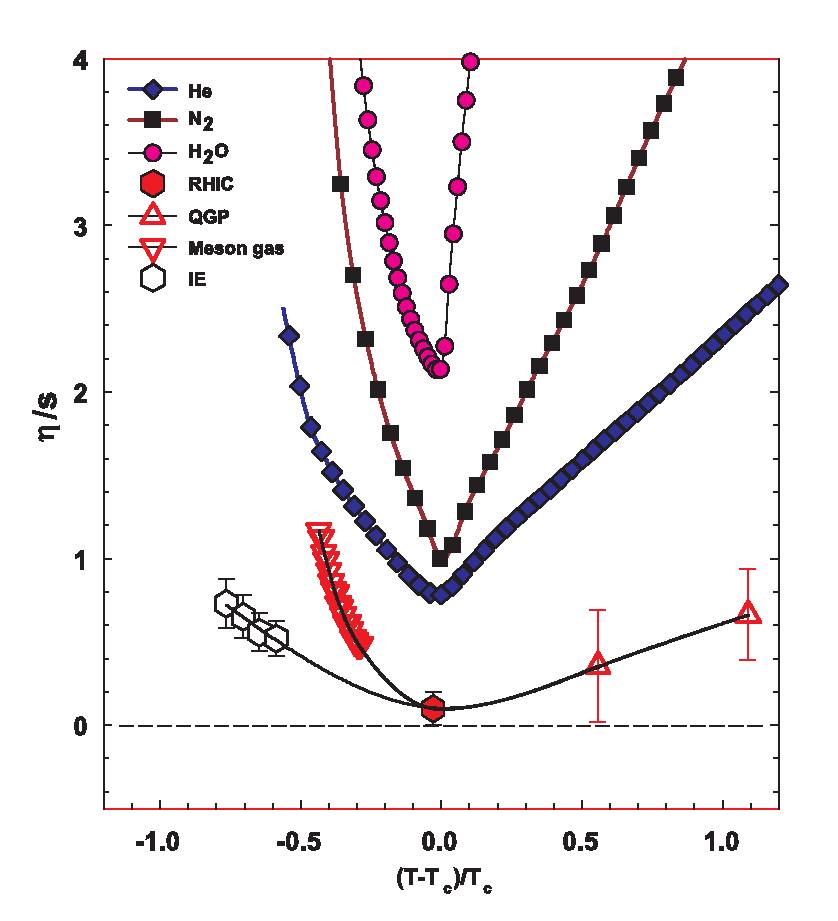
\includegraphics[width=0.5\textwidth]{pics/eta-s-vs-t-tc3}
\caption[$\eta/s$ vs $(T-T_c)/T_c$]{\label{fig3}$\eta/s$ as a function of $(T-T_c)/T_c$ for several substances as indicated.
	The calculated values for the meson-gas have an associated error 
	of $\sim$ 50\% %~\cite{Chen:2006ig}. 
	The lattice QCD value $T_c = 170$~MeV %~\cite{Karsch:2000kv} 
	is assumed for nuclear matter. The lines are drawn to guide the eye.~\cite{PhysRevLett.98.092301}
}
\label{fig:etas}
\end{figure}



\FloatBarrier
\pagebreak
\subsection{heavy-ion physics}
The Quark Gluon Plasma (QGP) is experimentally accessible by colliding heavy-ions at high energies. Nowadays research of Heavy-Ion Collisions is mainly performed at two particle colliders; The Relativistic heavy-ion Collider (RHIC) at BNL in New York, USA and he Large Hadron Collider (LHC) at CERN in Switzerland. Energy densities at these colliders should be enough to produce QGP and convincing evidence of the creation has been seen at both colliders.

The development of heavy-ion physics is strongly connected to the development of particle colliders. Experimental study of relativistic heavy-ion collisions has been carried out for three decades, beginning with the Bevalac at Lawrence Berkeley National Laboratory (LBNL)~\cite{Lofgren_1975}, and continuing with the AGS at Brookhaven National Laboratory (BNL)~\cite{Barton:1987}, CERN SPS~\cite{Vitev:2002pf}, RHIC at BNL and LHC at CERN. 

%The first colliders could not produce enough energy to create QGP matter so they could only probe the hadronic state. 
%
%The collective motion of matter in a heavy-ion collision has been modeled using several models e.g. the Blast wave Model~\cite{PhysRevC.84.064905} has been used succesfully. Another model growing in popularity is the hydrodynamical approach which is further discussed in section \ref{sec:hydro}.

\subsubsection{History}
The first heavy-ion collisions were performed at the Bevalac experiment at the Lawrence Berkeley National Laboratory~\cite{Lofgren_1975} and at the Joint Institute for Nuclear Research in Dubna~\cite{kovalenko1994status} at energies up to 1$\gev$ per nucleon.
In 1986 the Super Proton Synchrotron (SPS) at CERN started to look for QGP signatures in O+Pb collisions. The center-of-mass energy per colliding nucleon pair $\left(\sqrt{s_{NN}}\right)$ was \unit[19.4]{GeV}~\cite{Vitev:2002pf}. These experiments did not find any decisive evidence of the existence of QGP. In 1994 a heavier lead (Pb) beam was introduced for new experiments at $\sqrt{s_{NN}}\approx \unit[17]{\gev}$. At the same time the Alternating Gradient Synchrotron (AGS) at BNL, Brookhaven collided ions up to $\mathrm{^{32}S}$ with a fixed target at energies up to \unit[28]{\gev}~\cite{Barton:1987}. Although the discovery of a new state of matter was reported at CERN, these experiments provided no conclusive evidence of QGP. Now SPS is used with 400 GeV proton beams for fixed-target experiments, such as the SPS heavy-ion and Neutrino Experiment (SHINE)~\cite{Grebieszkow:2013nza}, which tries to search for the critical point of strongly interacting matter.

The Relativistic heavy-ion Collider (RHIC) at BNL in New York, USA started its  operation in 2000. The top center-of-mass energy per nucleon pair at RHIC, 200 GeV, was reached in the following years. The results from the experiments at RHIC have provided a lot of convincing evidences that QGP was created~\cite{Adcox:2004mh, Adams:2005dq, Arsene:2004fa, Back:2004je}. The newest addition to the group of accelerators capable of heavy-ion physics is the Large Hadron Collider (LHC) at CERN, Switzerland. LHC started operating in November 2009 with proton-proton collisions. First Pb-Pb heavy-ion runs started in November 2010 with $\sqrt{s_{NN}}=2.76\; \mathrm{TeV}$,  over ten times higher than at RHIC. Among the six experiments at LHC, the Large Ion Collider Experiment (ALICE) is dedicated to heavy-ion physics. Also CMS and ATLAS have active heavy-ion programs. 

{\color{red} add a table of LHC runs related ALICE}

\pagebreak
\FloatBarrier
%\pagebreak
\subsection{Features of Heavy-Ion Collisions}
\label{sec:features}
\subsubsection{Collision Geometry}
In contrast to protons atomic nuclei are objects with considerable transverse size. The properties of a heavy-ion collision depend strongly on the impact parameter $b$ which is the vector connecting the centers of the two colliding nuclei at their closest approach. One illustration of a heavy-ion collision is shown in Fig.~\ref{fig:planes}.


Impact parameter defines the reaction plane which is the plane spanned by $b$ and the beam direction. $\Psi_{RP}$ gives the angle between the reaction plane and some reference frame angle. Experimentally the reference frame is fixed by the detector setup. Reaction plane angle cannot be directly measured in high energy nuclear collisions, but it can be estimated with the event plane method~\cite{Voloshin:2008dg}. 
\begin{figure}[h!]
\centering
\includegraphics[width=0.6\textwidth]{pics/Definitions}
\caption[The definitions of the Reaction Plane and Participant Plane coordinate systems]{The definitions of the Reaction Plane and Participant Plane coordinate systems~\cite{Voloshin:2007pc}. The dashed circles represent the two colliding nuclei and the green dots are partons that take part  in the collision. $x_{PP}$ and $x_{RP}$ are the participant and reaction planes. The angle between $x_{RP}$ and $x_{PP}$ is given by Eq. (\ref{eq:partangle}). $y_{PP}$ and $y_{RP}$ are lines perpendicular to the participant and reaction planes. }
\label{fig:planes}
\end{figure}


%The constituents in the nucleus have a quantum character and are situated in a potential well. 
%Nucleus density
%This causes fluctuations in the initial geometry of the overlapping region. 
Participant zone is the area containing the participants. The distribution of nucleons in the nucleus exhibits time-dependent fluctuations. Because the nucleon distribution at the time of the collision defines the participant zone, the axis of the participant zone fluctuates and can deviate from the reaction plane. The angle between the participant plane and the reaction plane is defined by ~\cite{Holopainen:2010gz}

\begin{equation}
\psi_{PP}=\arctan \frac{-2\sigma_{xy}}{\sigma_y^2-\sigma_x^2+\sqrt{\left(\sigma_y^2-\sigma_x^2\right)^2+4\sigma_{xy}^2}},
\label{eq:partangle}
\end{equation}

\noindent where the $\sigma$-terms are averaged over the energy density.

\begin{equation}
\sigma_y^2=\langle y^2\rangle-\langle y \rangle ^2, \sigma_x^2=\langle x^2\rangle-\langle x \rangle ^2, \sigma_{xy}=\langle xy \rangle - \langle x \rangle \langle y \rangle
\end{equation}

The impact parameter is one way to quantize the centrality of a heavy-ion collision but it is impossible to measure in a collision. It can be estimated from observed data using theoretical models, but this is always model-dependent and to compare results from different experiments one needs an universal definition for centrality. The difference between central and peripheral collisions is illustrated in Fig.~\ref{fig:collisionA}. In a central collision the overlap region is larger than in a peripheral collision. Larger overlap region translates into a larger number of nucleons participating in the collision, which in turn leads to a larger number of particles produced in the event.


\begin{figure}[h!]
\centering
        \begin{subfigure}[b]{0.45\textwidth}
                \centering
            	\includegraphics[height=1in]{pics/Collisionperipheral}
                \caption{Peripheral collision}
                \label{fig:peripheral}
        \end{subfigure}
        \begin{subfigure}[b]{0.45\textwidth}
                \centering
               \includegraphics[height=1in]{pics/Collisioncentral}
                \caption{Central collision}
                \label{fig:central}
        \end{subfigure}
        \caption[Interaction between partons in central and peripheral collisions.]{Interaction between partons in central and peripheral collisions. The snowflakes represent elementary parton-parton collisions. When the impact parameter $b$ is large the number of elementary collisions is small. Particle production is small. Smaller impact parameter increases the number of elementary collisions. This increases  particle production.}\label{fig:collisionA}
\end{figure}

Usually centrality is defined by dividing collision events into percentile bins by the number participants or experimentally by the observed multiplicity. Centrality bin 0-5\% corresponds to the most central collisions with the highest multiplicity and higher centrality percentages correspond to more peripheral collisions with lower multiplicities. A multiplicity distribution from ALICE measurements~\cite{PhysRevC.88.044909} illustrating the centrality division is shown in Fig.~\ref{fig:centrality}. The distribution is fitted using a phenomenological approach based on a Glauber Monte Carlo~\cite{Miller:2007ri} plus a convolution of a model for the particle production and a negative binomial distribution. 


\begin{figure}[htb]
\centering

               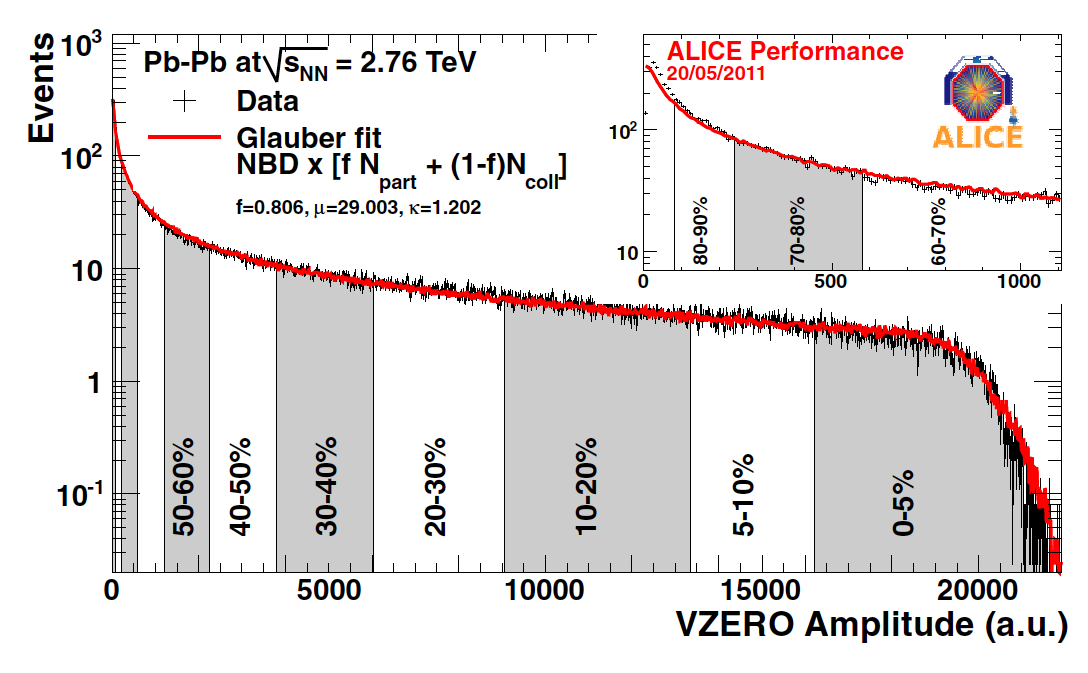
\includegraphics[width=0.9\textwidth]{pics/centrality.png}
        \caption[An illustration of the multiplicity distribution in ALICE measurement with centrality classes.]{An illustration of the multiplicity distribution in ALICE measurements. The red line shows
the fit of the Glauber calculation to the measurement. The data is divided into centrality bins~\cite{PhysRevC.88.044909}. The size of the bins corresponds to the indicated percentile.}
        	\label{fig:centrality}
\end{figure}

%Each centrality bin is obtained by taking the indicated percentile of events arranged by the observed multiplicity. 
%Centrality bin 0-5\% corresponds to the most central collisions. It includes the 5\% of the events  with highest multiplicity. Centralities 90-100\% correspond to the most peripheral collisions. 


\subsubsection{Nuclear Geometry}
\label{sec:glauber}
To model heavy-ion collisions one must first have a description as good as possible of the colliding objects. Atomic nuclei are complex ensembles of nucleons. The nuclei used in heavy-ion physics have in the order of 200 nucleons. Mostly used nuclei are $\mathrm{^{208}Pb}$ at LHC and $\mathrm{^{197}Au}$ at RHIC. The distribution of these nucleons within a nucleus is not uniform and is subject to fluctuations in time.

Nuclear geometry in heavy-ion collisions is often modelled with the Glauber Model. The model was originally developed to address the problem of high energy scattering with composite particles. Glauber presented his first collection of papers and unpublished work in his 1958 lectures~\cite{Glauber:1959}. In the 1970's Glauber's work started to have utility in describing total cross sections. Maximon and Czyz applied it to proton-nucleus and nucleus-nucleus collisions in 1969~\cite{Czyz:1969}. 

In 1976 ~\cite{Biallas1976461} Białłas, Bleszyński, and Czyż applied Glauber's approach to inelastic nuclear collisions. Their approach introduced the basic functions used in modern language including the thickness function and the nuclear overlap function. Thickness function is the integral of the nuclear density over a line going through the nucleus with minimum distance $s$ from its center

\begin{equation}
T_A\left(s\right)=\int_{-\infty}^{\infty}\dd z \rho\left(\sqrt{s^2+z^2}\right).
\end{equation}

\noindent This function gives the thickness of the nucleus, i.e. the amount material seen by a particle passing through it. 

Overlap function is an integral of the thickness functions of two colliding nuclei over the overlap area. This can be seen as the material that takes part in the collision. It is given as a function of the impact parameter $b$

\begin{equation}
T_{AB}\left(b\right)=\int \dd  s^2 T_A\left(\bar s\right) T_B\left(\bar s - \bar b\right)
\end{equation}

\noindent The average overlap function, $\left<T_{AA}\right>$, in an A-A collisions  is given by~\cite{Afanasiev:2009aa}

\begin{equation}
\left<T_{AA}\right>=\frac{\int T_{AA}\left(b\right) \dd b}
{\int\left(1-e^{-\sigma^{inel}_{pp}T_{AA}\left(b\right)}\right)\dd b}.
\end{equation}

\noindent Using $\left<T_{AA}\right>$ one can calculate the mean number of binary collisions

\begin{equation}
\left<N_{coll}\right>=\sigma_{pp}^{inel}\left<T_{AA}\right>,
\end{equation}

\noindent where the total inelastic cross-section, $\sigma_{pp}^{inel}$, gives the probability of two nucleons interacting. The number of binary collisions is related to the hard processes in a heavy-ion collision. Each binary collision has equal probability for direct production of high-momentum partons. Thus the number of high momentum particles is proportional to $\left<N_{coll}\right>$.

Soft production on the other hand is related to the number of participants. It is assumed that in the binary interactions participants get excited and further interactions are not affected by previous interactions because the time scales are too short for any reaction to happen in the nucleons. After the interactions excited nucleons are transformed into soft particle production. Production does not depend on the number of interactions a nucleon has gone through. The average number of participants, $\left<N_{part}\right>$ can also be calculated from the Glauber model 


\begin{eqnarray}
\left<N_{part}^{AB}\left(b\right)\right>&=&\int \dd  s^2 T_A\left(\bar s\right)\left[1-\left[1-\sigma_{NN}\frac{T_B\left(\bar s - \bar b\right)}{B}\right]^B\right] \nonumber \\
 &+ &\int \dd s^2 T_B\left(\bar s\right)\left[1-\left[1-\sigma_{NN}\frac{T_A\left(\bar s - \bar b\right)}{A}\right]^A\right].
\end{eqnarray}

%
%
%
%
%The mean number of binary nucleon collisions can be calculated from the average thickness function 
%
%\begin{equation}
%\left<N_{coll}\right>=\sigma_{pp}^{inel}\left<T_{AA}\right>
%\end{equation}
%
%where $\left<T_{AA}\right>$ is the mean Glauber overlap function for the centrality being analysed 
%
%\begin{equation}
%\left<T_{AA}\right>=\frac{\int T_{AA}\left(b\right)}{\int\left(1-e^{-\sigma^{inel}_{pp}T_{AA}\left(b\right)}\right)db}.
%\end{equation}
%
%
%
%Number of participants is related to the bulk production / soft production. 
%


Glauber calculations require some knowledge of the properties of the nuclei. One requirement is the nucleon density distribution, which can be experimentally determined by studying the nuclear charge distribution in low-energy electron scattering experiments~\cite{Miller:2007ri}.  The nucleon density is usually parametrized by a Woods-Saxon  distribution

%\begin{equation}
%\rho\left(r\right)=\rho_0 \frac{1+w\left(\frac{r}{R}\right)^2}{1+\exp{\left(\frac{r-R}{a}\right)}}
%,\end{equation}
%
\begin{equation}
\rho\left(r\right)=\frac{\rho_0}{1+\exp{\left(\frac{r-R}{a}\right)}}
,\end{equation}

\noindent where $\rho_0$ is the nucleon density in center of the nucleus, $R$ is the nuclear radius and $a$ parametrizes the depth of the skin. The density stays relatively constant as a function of $r$ until around $R$ where it drops to almost 0 within a distance given by $a$.

Another observable required in the calculations is the total inelastic nucleon-nucleon cross-section $\sigma\mathrm{^{NN}_{inel}}$.  This can be measured in proton-proton collisions at different energies.

There are two often used approaches to Glauber calculations. The optical approximation is one way to get simple analytical expressions for the nucleus-nucleus interaction cross-section, the number of interacting  nucleons and the number of nucleon-nucleon collisions. In the optical Glauber it is assumed that during the crossing of the nuclei the nucleons move independently and they will be essentially undeflected.  

With the increase of computational power at hand the Glauber Monte Carlo (GMC) approach has emerged as a method to get a more realistic description of the collisions. In GMC the nucleons are distributed randomly in three-dimensional coordinate system according to the nuclear density distributions. Also nuclear parameters, like the radius $R$ can be sampled from a distribution. A heavy-ion collision is then treated as a series of independent nucleon-nucleon collisions, where in the simplest model nucleons interact if their distance  in the plane orthogonal to the beam axis, $d$, satisfies

\begin{equation}
d< \sqrt{\sigma\mathrm{^{NN}_{inel}}}
\end{equation}

\noindent The average number of participants and binary collisions can then be determined by simulating many nucleus-nucleus collisions. The results of one GMC Pb-Pb event with impact parameter $b=\unit[9.8]{fm}$ is shown in Fig.~\ref{fig:GMC}

\begin{figure}[htbp]
\centering
               \includegraphics[width=0.5\textwidth]{pics/glauber_eli}
        \caption[The results of one Glauber Monte Carlo simulation.]{The results of one Glauber Monte Carlo simulation. Big circles with black dotted boundaries represent the two colliding nuclei. The participant zone is highlighted with the solid red line.        
        Small red and blue circles represent nucleons. Circles with thick boundaries are participants i.e. they interact with at least one nucleon from the other nucleus. Small circles with dotted boundaries are spectators which do not take part in the collision.}
        	\label{fig:GMC}
\end{figure}



\subsubsection{Hydrodynamical Modelling}
\label{sec:hydro}
The relativistic version of hydrodynamics has been used to model the deconfined phase of a heavy-ion collision with success. Heavy-ion collisions produce many hadrons going into all directions. It is expected that tools from statistical physics would be applicable to this complexity~\cite{Ollitrault:2007du}. The power of relativistic hydrodynamics lies in its simplicity and generality. Hydrodynamics only requires that there is local thermal equilibrium in the system. In order to reach thermal equilibrium the system must be strongly coupled so that the mean free path is shorter than the length scales of interest~\cite{Romatschke:2009im}.

The use of relativistic hydrodynamics in high-energy physics dates back to Landau~\cite{Landau:1953gs} and the 1950's, before QCD was discovered. Back then it was used in proton-proton collisions. Development of hydrodynamics for the use of heavy-ion physics has been active since the 1980's, including Bjorken's study of boost-invariant longitudinal expansion and infinite transverse flow~\cite{PhysRevD.27.140}. Major steps were taken later with the inclusion of finite size and and dynamically generated transverse size~\cite{Baym:1984sr, PhysRevD.34.794}, a part of which was done at the University of Jyväskylä. The role of hydrodynamics in heavy-ion physics was strengthened when QGP was observed to behave like a liquid by RHIC~\cite{Adcox:2004mh}. 

The evolution of a heavy-ion event can be divided into four stages. A schematic representation of the evolution of the collisions is shown in Fig.~\ref{fig:HISpaceTime}. Stage 1 follows immediately the collision. This is known as the pre-equilibrium stage. Hydrodynamic description is not applicable to this regime because thermal equilibrium is not yet reached. The length of this stage is not known but it is assumed to last about $1\ \mathrm{fm}/c$ in proper time $\tau$. 

\begin{figure}[htb]
\centering
               \includegraphics[width=0.5\textwidth]{pics/HISpaceTime2}
        \caption[Schematic representation of a heavy-ion collision]{Schematic representation~\cite{Romatschke:2009im} of a heavy-ion collision as the function of time and longitudinal coordinates $z$ The various stages of the evolution correspond to proper time $\tau=\sqrt{t^2-z^2}$ which is shown as hyperbolic curves separating the different stages.}
        	\label{fig:HISpaceTime}
\end{figure}

The second stage is the regime where thermal equilibrium or at least near-equilibrium is reached. In this stage hydrodynamics should be applicable if the temperature is above the deconfinement temperature~\cite{Romatschke:2009im}. This lasts about $5-10\ \mathrm{fm}/c$ until the temperature of the system sinks low enough for hadronization to occur. Now the system loses its deconfined, strongly coupled, state and hydrodynamics can no longer be used. The third stage is the hadron gas stage where the hadrons still interact. This ends when hadron scattering becomes rare and they no longer interact. In the final stage hadrons are free streaming and they fly in straight lines until they reach the detector.

%The hydrodynamical approach uses. Mass density is not a well defined quantity since pair production and annihilation of quark-antiquark pairs constantly modifies the mass of the system. Instead energy density is used. 

The hydrodynamical approach treats the ensemble of particles as a fluid. It uses  basic equations from hydrodynamics and thermodynamics but with a few modifications to account for the relativistic energies. The calculation is based on a collection of differential equations connecting the local thermal variables like temperature, pressure etc. to local velocities of the fluid. One also needs equations of state that connect the properties of the matter, e.g. temperature and pressure to density.  Given initial conditions and equations of state the calculation gives the time-evolution of the system.

At first only ideal hydrodynamics was used. Ideal hydrodynamics does not include viscosity but it is a relatively good approximation and it could predict phenomena like elliptic flow. For more detailed calculations also viscosity must be considered and viscosity itself is an interesting property of QGP.


\FloatBarrier
\pagebreak
\subsection{Flow}
In a heavy-ion collision the bulk particle production is known as flow. The production is mainly isotropic but a lot of studies including my thesis focus on the small anisotropies. After the formation of the QGP, the matter begins to expand as it is driven outwards by the strong pressure difference between the center of the collision zone and the vacuum outside the collision volume. The pressure-driven expansion is transformed into flow of low-momentum particles in the hadronization phase. Since the expansion is mainly isotropic the resulting particle flow is isotropic with small anisotropic corrections that are of the order of $10\%$ at most. The isotropic part of flow is referred to as radial flow. 

\begin{figure}[b!]
\centering
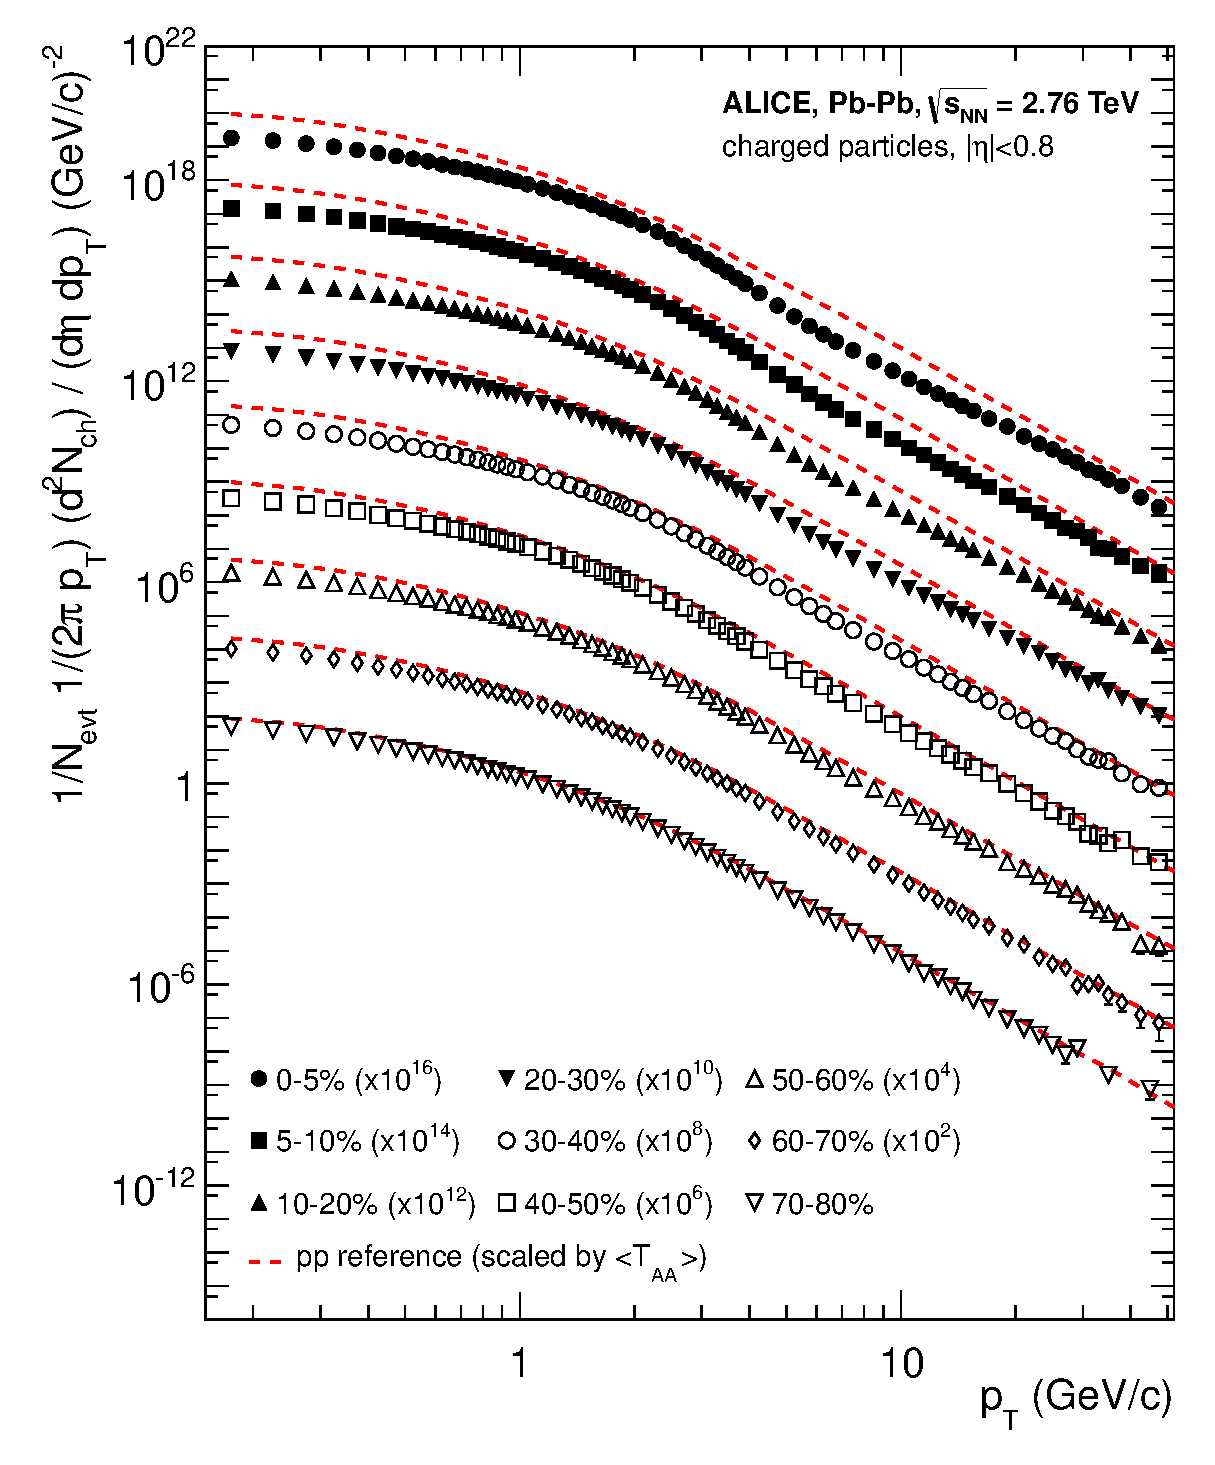
\includegraphics[width=0.6\textwidth]{pics/pT_PbPb}
\caption[Charged particle spectra]{ Charged particle spectra measured by ALICE~\cite{PRL106032301} for the 9 centrality classes given in the legend. The distributions are offset by arbitrary factors given in the legend for clarity. The distributions are offset by arbitrary factors given in the legend for clarity. The dashed lines show the proton-proton reference spectra scaled by the nuclear overlap function determined for each centrality class and by the Pb-Pb spectra scaling factors~\cite{PRL106032301}.}
\label{fig:dndpt}
\end{figure}

The transverse momentum spectra $\dd N/\dd {\pt{}}$ in heavy-ion collisions is shown in Fig. \ref{fig:dndpt}. The vast majority of produced particles have small $\pt{}$. The difference between the yield of $1\gevc$ and $4\gevc$ particles is already 2-3 orders of magnitude. Any observables that are integrated over $\pt{}$ are therefore dominated by the small momentum particles.




\subsubsection{Anisotropic Flow}
In a non-central heavy-ion collision the shape of the impact zone is almond-like. In peripheral collisions the impact parameter is large which means a strongly asymmetric overlap region.  In a central collision the overlap region is almost symmetric in the transverse plane. In this case the impact parameter is small. Collisions with different impact parameters are shown in Fig.~\ref{fig:collisionA}.

\begin{figure}[b!]
\centering
        \begin{subfigure}[b]{0.52\textwidth}
                \centering
            	\includegraphics[height=2.4in]{pics/InteractionB}
                \caption{Peripheral collision}
                \label{fig:InteractionB}
        \end{subfigure}
        \begin{subfigure}[b]{0.45\textwidth}
                \centering
               \includegraphics[height=2.4in]{pics/InteractionA}
                \caption{Central collision}
                \label{fig:InteractionA}
        \end{subfigure}
	\caption[Illustration of flow in momentum space in central and peripheral collisions.]{Illustration of flow in momentum space in central and peripheral collisions. The density of the arrows represent the magnitude of flow seen at a large distance from the collision in the corresponding azimuthal direction. In a peripheral collision momentum flow into in-plane direction is strong and flow into out-of-plane direction is weak. In a central collision anisotropy in flow is smaller, but the total yield of particles is larger.}
	\label{fig:flow}
\end{figure}

The pressure gradient is largest in-plane, in the direction of the impact parameter $b$, where the distance from high pressure, at the collision center, to low pressure, outside the overlap zone, is smallest. This leads to stronger collective flow into in-plane direction, which in turn results in enhanced thermal emission through a larger effective temperature into this direction, as compared to out-of-plane~\cite{Ollitrault:1992,Ollitrault:1993, Heinz:2002}. The resulting flow is illustrated in Fig.~\ref{fig:flow}. Flow with two maxima in the direction of the reaction plane is called elliptic flow. This is the dominant part of anisotropic flow. Also more complex flow patterns can be identified. The most notable of these is the triangular flow, which is mainly due to fluctuations in the initial conditions.

Flow is nowadays usually quantified in the form of a Fourier composition 

\begin{equation}
E\frac{\dd{^3N}}{\dd {p^3}}=\frac{1}{2\pi}\frac{\dd {^2N}}{\pt{ }\dd {\pt{ }}\dd {\eta} } \left(1+\sum_{n=1}^{\infty}2v_n\left(\pt{},\eta\right)\cos(n(\phi-\Psi_n))\right),
%\label{eq:finalseries}
\end{equation}

\noindent where the coefficients $v_n$ give the relative strengths of different anisotropic flow components and the overall normalisation gives the strength of radial flow. Elliptic flow is represented by $v_2$ and $v_3$ represents triangular flow. The first coefficient, $v_1$, is connected to directed flow. This will however in total be zero because of momentum conservation. It can be nonzero in some rapidity or momentum regions but it must be canceled by other regions.

The first approaches to quantifying the anisotropy of flow did not use the Fourier composition. Instead they approached the problem with a classic event shape analysis using directivity~\cite{danielewicz:1985} or sphericity~\cite{Ollitrault:1992, Danielewicz:1983283} to quantify the flow.


%The first one to predict anisotropic flow in heavy-ion collisions was Ollitrault in 1992~\cite{Ollitrault:1992}. The first papers on anisotropy did not discuss the Fourier composition. Instead they approached the problem with an classic event shape analysis. (sphericity)

The first experimental studies of anisotropy were performed at the AGS~\cite{PhysRevLett.70.1393} in 1993. They noted that the anisotropy of particle production in one region correlates with the reaction plane angle defined in another region. 

The first ones to present the Fourier decomposition were Voloshin and Zhang in 1996~\cite{Voloshin:1994mz}. This new approach was useful for detecting different types of anisotropy in flow, since the different Fourier coefficients give different harmonics in flow. They also show the relative magnitude of each harmonic compared to radial flow.

Some parts of the Fourier composition approach were used for Au-Au collisions at $\snn=11.4\gev$ at AGS in 1994~\cite{Barrette:1994xr}. This analysis still focused on event shapes but they constructed these shapes using Fourier composition from different rapidity windows.


{\color{red} Add a paragraph on the lessions learned from flow studies.}

\FloatBarrier

%\subsubsection{High $\pt{}$ Phenomena}
%The measurement of anisotropic flow coefficients can be extended to very high transverse momenta $\pt{}$. High $\pt{}$ measurements of $v_2$ from CMS~\cite{Chatrchyan:2012xq} are shown in Fig. \ref{fig:highpt}. For high transverse momenta $v_2$ values are positive and they decrease slowly as a function of $\pt{}$. At high transverse momentum the $v_2$ values don't, however, represent flow. 

\FloatBarrier
%\subsubsection{Fluctuations and Event-by-Event Flow}
%The colliding nuclei are not static objects but the distribution of nucleons fluctuates over time. The arrangement of the nucleons at the time of the collision is random, which leads to fluctuations in the initial conditions. The shape of the collision zone is not a perfect almond and it can have a more complex shape. Also the density of the created medium is not homogenous but it can have dense hot spots. The initial density distribution of the created medium is the main reason for anisotropic flow. Because of fluctuations the strength of anisotropic flow is not constant event-by-event.
%
%The existence of more complex density profiles also leads to odd flow harmonics. The basic hydrodynamical approach could only explain elliptic flow and even-harmonics. For a long time it was believed that the odd harmonics would be negligible. In 2007 Mishra {\emph et al.}~\cite{Mishra:2007tw} argued that density inhomogeneities in the initial state would lead to non-zero $v_n$ values for higher harmonics including $v_3$.  It was later noted that higher harmonics of $v_n$ would be suppressed by viscous effects and that the shape of $v_n$ as a function of $n$ would provide another valuable tool for studying $\eta/s$~\cite{Mocsy:2010um}. 
%
%In 2010 significant $v_3$ components were also observed in RHIC data~\cite{Alver:2010gr}. The AMPT model that is also studied in this thesis was able to quantitatively describe the centrality dependence of $v_3$ at RHIC and LHC energies, $\snn=200 \gev$ and $2.76\tev$~\cite{Xu:2011fe}.
%
%%Initial state fluctuations can be modelled using the Glauber model~\cite{Alver:2008zza}. However, so far all models fail to describe the experimental $v_n$ distributions consistently over the whole centrality range~\cite{Jia:2012ve}.
%
%Contrary to elliptic flow higher harmonics are not strongly affected by the centrality of the collision. This supports the theory of higher harmonics being the result of fluctuations. Also $v_2$ measurements of ultra-central collisions give non-zero results for flow, even though the traditional approach based on the anisotropy of the overlap zone gives no prediction of anisotropic flow. This is also the result of fluctuations. Measurement of distributions of $v_n$ coefficients has been performed at ATLAS~\cite{Jia:2012ve}. Their measurements of distributions for $v_2$ in central collisions and for $v_3$ and $v_4$ in general are consistent with a pure Gaussian fluctuation scenario~\cite{Jia:2012ve}.
%
%\begin{figure}[tb]
%	\centering
%	\begin{subfigure}[t]{0.5\textwidth}
%                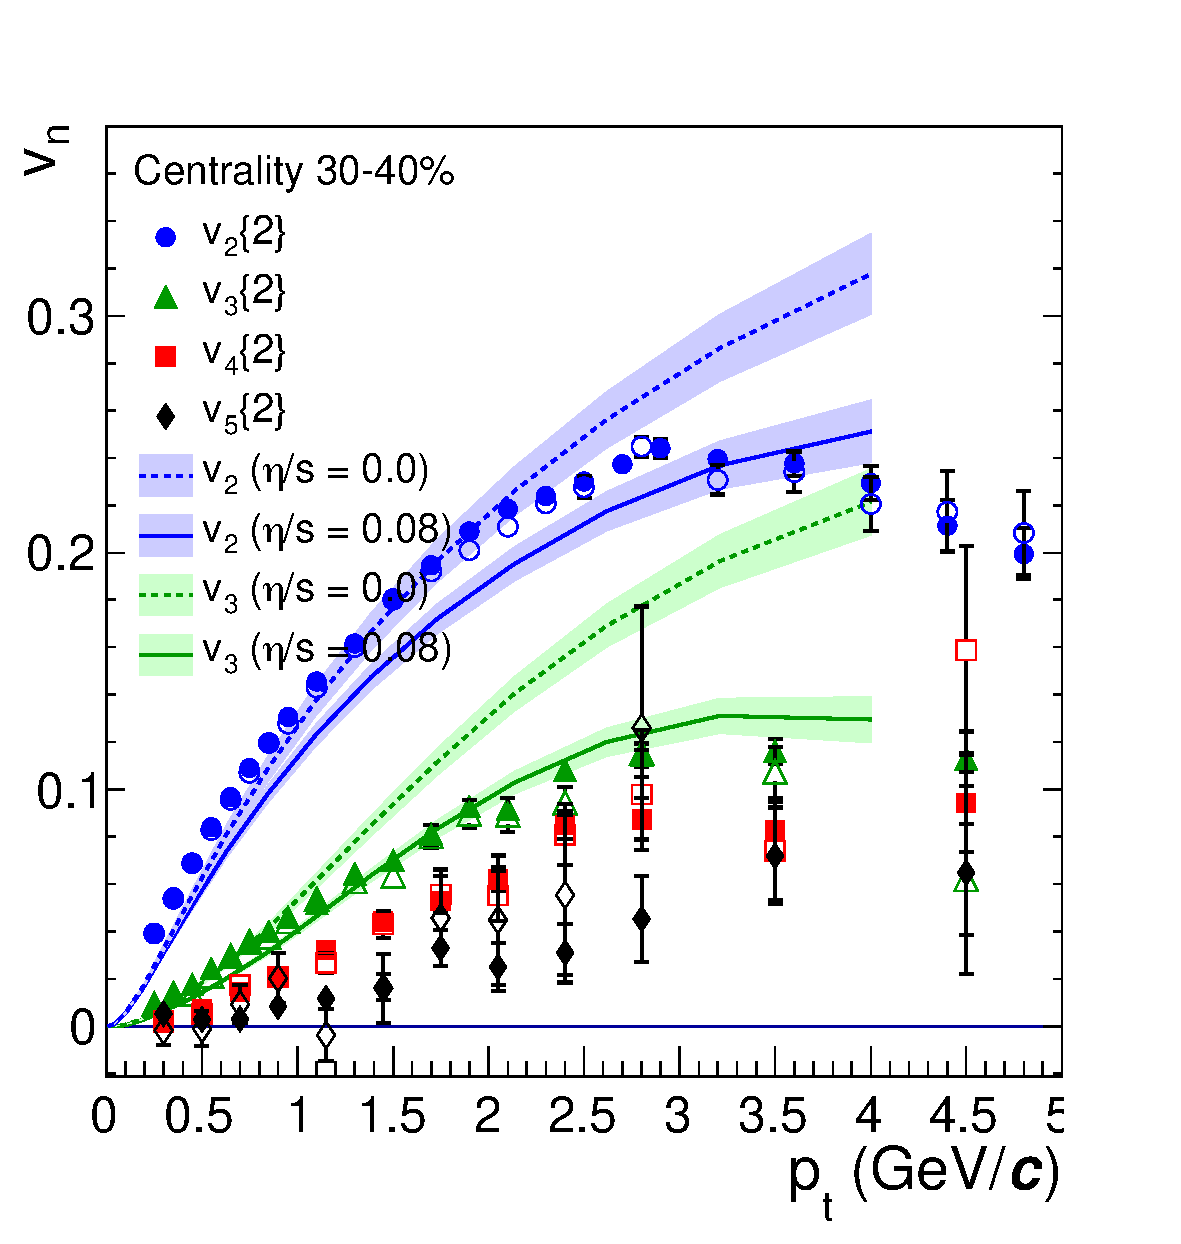
\includegraphics[width=\textwidth]{pics/alice_vn_figa.pdf}
%        \caption[ALICE measurement of $v_2$, $v_3$, $v_4$, $v_5$]{ALICE measurement of $v_2$, $v_3$, $v_4$, $v_5$ as a function of transverse momentum. The flow coefficients are determined by two-particle correlations using different rapidity separations. 
%        The full and open symbols are for $\Delta\eta > 0.2$ and $\Delta\eta > 1.0$. 
%        The results are compared to hydrodynamic predictions~\cite{Schenke:2011tv} with different values of $\eta/s$~\cite{PRL107032301}.}
%        \label{fig:higherharmonics}
%        \end{subfigure}
%        \quad
%        \begin{subfigure}[t]{0.45\textwidth}
%        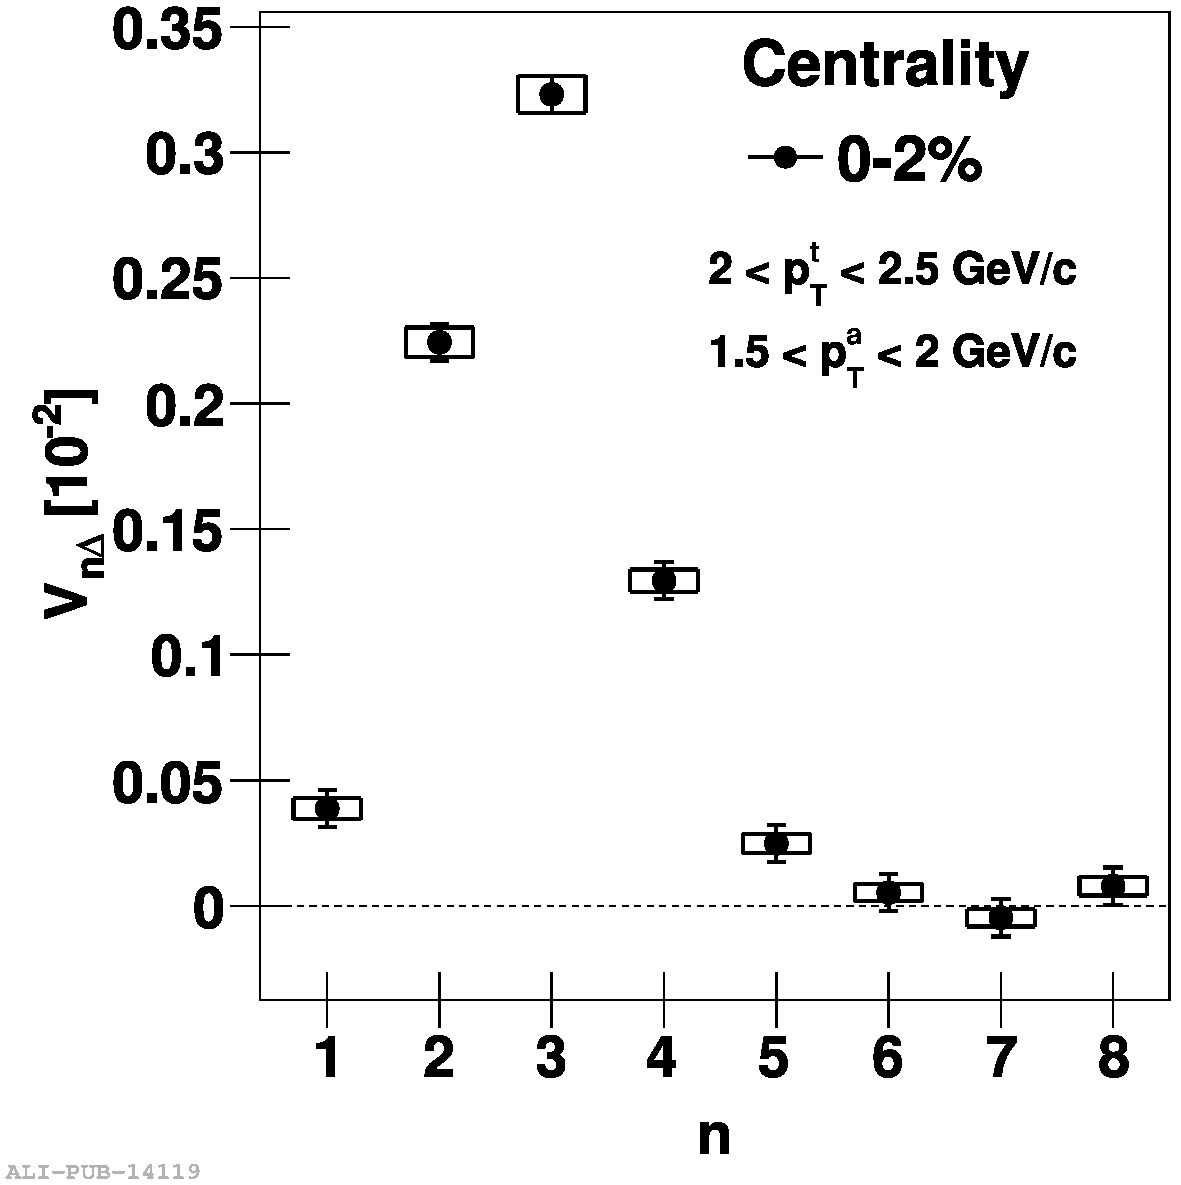
\includegraphics[width=\textwidth]{pics/2012-Jun-06-fig02b}
%        \caption{Amplitude of $v_n$ harmonics as a function of $n$ for the 2\% most central collisions as  measured by ALICE~\cite{Aamodt2012249}.}
%        \label{fig:alicepowers}
%
%        \end{subfigure} 
%        
%%        \begin{subfigure}[t]{\textwidth}
% %               \includegraphics[width=\textwidth]{pics/atlas_powerspectra.png}
%%        \caption{Power spectra of $v_n$ for the 1\% most central collisions measured by ATLAS~\cite{PhysRevC.86.014907}.}
%%        \label{fig:atlaspowers}
% %       \end{subfigure}
%                \caption[Flow measurements of higher harmonics]{Flow measurements of higher harmonics}
%                \label{fig:vnpowers}
%
%\end{figure}
%
%Measurements of different flow harmonics are shown in Fig.~\ref{fig:vnpowers}. The left panel shows different flow harmonics as a function of $\pt{}$ as measured by ALICE~\cite{PRL107032301} in peripheral collisions. In general flow coefficients decrease as a function of $n$ after $n=2$. Central collisions are an exception.The right panel of  Fig.~\ref{fig:vnpowers} shows $v_n$ as a function of $n$ in central collisions as measured by ALICE~\cite{Aamodt2012249}.
%
%
%
%Measurement of event-by-event flow and higher harmonics has growing importance in the field. Triangular flow is useful also for studying jet quenching and in-medium energy loss since anisotropies of flow are related to the path lengths of partons traversing through the medium. Path-lengths and medium density in turn are related the energy loss. An interesting topic of future research would be studying jet properties like $R_{AA}$ separately in events with strong and weak anisotropy.

\subsection{Hard processes}
\subsubsection{pQCD factorization}


%\begin{figure}[htb]
%\centering
%\includegraphics[width=0.5\textwidth]{pics/QCDLO}
%\caption[QCD Leading Order]{The basic pQCD processes and their quadratic matrix elements}
%\label{fig:qcdlo2}
%\end{figure}


\begin{figure}[htb]
\centering
\documentclass{standalone}
\usepackage{tikz}
\usepackage{array}
\usetikzlibrary{shapes,arrows}
\usetikzlibrary{trees}
\usetikzlibrary{shadows.blur}
\usetikzlibrary{positioning}
\usetikzlibrary{decorations.pathmorphing}
\usetikzlibrary{decorations.markings}
\begin{document}
\newcommand{\centered}[1]{\begin{tabular}{l} #1 \end{tabular}}

\tikzset{
photon/.style={decorate, decoration={snake}, draw=red},
particlearrow/.style={draw=black, postaction={decorate},
    decoration={markings,mark=at position .5 with {\arrow[draw=black]{>}}}},
antiparticlearrow/.style={draw=black, postaction={decorate},
    decoration={markings,mark=at position .5 with {\arrow[draw=black]{>}}}},
particle/.style={draw=black},
antiparticle/.style={draw=blue},
gluon/.style={decorate, draw=black,
    decoration={coil,amplitude=2pt, segment length=3pt}}
 }
 
%\begin{tabular}{ >{\centering\arraybackslash} m{2cm} >{\centering\arraybackslash} m{2cm} >{\centering\arraybackslash} m{8cm}}
\begin{tabular}{ c c c}

\begin{tabular}{c}
$qq' \rightarrow qq' $ \\
$\bar q q' \rightarrow \bar qq' $
\end{tabular} 
& $\frac{4}{9}\frac{\hat s^2+\hat u^2}{\hat t^2}$

&
\centered{

 \begin{tikzpicture}[node distance=1cm and 1.5cm]
\coordinate[] (e1);
\coordinate[right=1cm of e1] (aux1);
\coordinate[right=1cm of aux1] (e2);
\coordinate[below=1cm of aux1] (aux2);
\coordinate[left=1cm of aux2] (e3);
\coordinate[right=1cm of aux2] (e4);

\draw[particle] (e1) -- (aux1);
\draw[particle] (aux1) -- (e2);
\draw[particle] (e3) -- (aux2);
\draw[particle] (aux2) -- (e4);
\draw[gluon] (aux2) -- node[label=left:$t$] {} (aux1);
\end{tikzpicture} 

}
 \\
$qq \rightarrow qq$ & $\frac{4}{9}\left( \frac{\hat s^2+\hat u^2}{\hat t^2} + \frac{\hat s^2+\hat u^2}{\hat t^2}  \right) - \frac{8}{27}\frac{\hat s^2}{\hat u \hat t}$ &
\centered{

\begin{tikzpicture}[node distance=1cm and 1.5cm]
\coordinate[] (e1);
\coordinate[right=1cm of e1] (aux1);
\coordinate[right=1cm of aux1] (e2);
\coordinate[below=1cm of aux1] (aux2);
\coordinate[left=1cm of aux2] (e3);
\coordinate[right=1cm of aux2] (e4);

\draw[particlearrow] (e1) -- (aux1);
\draw[particlearrow] (aux1) -- (e2);
\draw[particlearrow] (e3) -- (aux2);
\draw[particlearrow] (aux2) -- (e4);
\draw[gluon] (aux2) -- node[label=left:$t$] {} (aux1);
\end{tikzpicture} 

\begin{tikzpicture}[node distance=1cm and 1.5cm]
\coordinate[] (e1);
\coordinate[right=1cm of e1] (aux1);
\coordinate[right=1cm of aux1] (e2);
\coordinate[below=1cm of aux1] (aux2);
\coordinate[left=1cm of aux2] (e3);
\coordinate[right=1cm of aux2] (e4);

\draw[particlearrow] (e1) -- (aux1);
\draw[particle] (aux1) -- (e4);
\draw[particlearrow] (e3) -- (aux2);
\draw[particle] (aux2) -- (e2);
\draw[gluon] (aux2) -- node[label=left:$u$] {} (aux1);
\end{tikzpicture}
}
\\
$\bar q q \rightarrow \bar q' q'$ & $\frac{4}{9}\frac{\hat t^2+\hat u^2}{\hat s^2}$ &
\centered{
\begin{tikzpicture}[node distance=1cm and 1.5cm]
\coordinate[] (e1);
\coordinate[below right=0.7cm of e1] (aux1);
\coordinate[right=1cm of aux1] (aux2);
\coordinate[above right=0.7cm of aux2] (e2);
\coordinate[below left=0.7cm of aux1] (e3);
\coordinate[below right=0.7cm of aux2] (e4);

\draw[antiparticlearrow] (aux1) -- (e1);
\draw[antiparticlearrow] (e2) -- (aux2);
\draw[particlearrow] (e3) -- (aux1);
\draw[particlearrow] (aux2) -- (e4);
\draw[gluon] (aux2) -- node[label=above:$s$] {} (aux1);
\end{tikzpicture}
}
\\
$\bar q q \rightarrow \bar q q$ & $\frac{4}{9}\left( \frac{\hat s^2+\hat u^2}{\hat t^2} + \frac{\hat t^2+\hat u^2}{\hat s^2}  \right) - \frac{8}{27}\frac{\hat u^2}{\hat s \hat t}$ &
\centered{

\begin{tikzpicture}[node distance=1cm and 1.5cm]
\coordinate[] (e1);
\coordinate[below right=0.7cm of e1] (aux1);
\coordinate[right=1cm of aux1] (aux2);
\coordinate[above right=0.7cm of aux2] (e2);
\coordinate[below left=0.7cm of aux1] (e3);
\coordinate[below right=0.7cm of aux2] (e4);

\draw[antiparticlearrow] (aux1) -- (e1);
\draw[antiparticlearrow] (e2) -- (aux2);
\draw[particlearrow] (e3) -- (aux1);
\draw[particlearrow] (aux2) -- (e4);
\draw[gluon] (aux2) -- node[label=above:$s$] {} (aux1);
\end{tikzpicture}
\begin{tikzpicture}[node distance=1cm and 1.5cm]
\coordinate[] (e1);
\coordinate[right=1cm of e1] (aux1);
\coordinate[right=1cm of aux1] (e2);
\coordinate[below=1cm of aux1] (aux2);
\coordinate[left=1cm of aux2] (e3);
\coordinate[right=1cm of aux2] (e4);

\draw[antiparticlearrow] (e2) -- (aux1);
\draw[antiparticlearrow] (aux1) -- (e1);
\draw[particlearrow] (e3) -- (aux2);
\draw[particlearrow] (aux2) -- (e4);
\draw[gluon] (aux2) -- node[label=left:$t$] {} (aux1);
\end{tikzpicture} 
}
\\
$\bar q q \rightarrow gg$ & $\frac{32}{27}\frac{\hat u^2+\hat t^2}{\hat u \hat t} - \frac{8}{3}\frac{\hat u^2 + \hat t^2}{\hat s^2}$ &
\centered{

\begin{tikzpicture}
\coordinate[] (e1);
\coordinate[below right=0.7cm of e1] (aux1);
\coordinate[right=1cm of aux1] (aux2);
\coordinate[above right=0.7cm of aux2] (e2);
\coordinate[below left=0.7cm of aux1] (e3);
\coordinate[below right=0.7cm of aux2] (e4);

\draw[antiparticlearrow] (aux1) -- (e1);
\draw[gluon] (aux2) -- (e2);
\draw[particlearrow] (e3) -- (aux1);
\draw[gluon] (aux2) -- (e4);
\draw[gluon] (aux2) -- node[label=above:$s$] {} (aux1);
\end{tikzpicture}
}
\\
$gg \rightarrow \bar q q$ & $\frac{1}{6}\frac{\hat u^2+\hat t^2}{\hat u \hat t} - \frac{3}{8}\frac{\hat u^2 + \hat t^2}{\hat s^2}$ &
\centered{

\begin{tikzpicture}
\coordinate[] (e1);
\coordinate[below right=0.7cm of e1] (aux1);
\coordinate[right=1cm of aux1] (aux2);
\coordinate[above right=0.7cm of aux2] (e2);
\coordinate[below left=0.7cm of aux1] (e3);
\coordinate[below right=0.7cm of aux2] (e4);

\draw[gluon] (e1) -- (aux1);
\draw[antiparticlearrow] (e2) -- (aux2);
\draw[gluon] (e3) -- (aux1);
\draw[particlearrow] (aux2) -- (e4);
\draw[gluon] (aux2) -- node[label=above:$s$] {} (aux1);
\end{tikzpicture}
}
\\

$q g  \rightarrow qg $ & $\frac{4}{9}\frac{\hat u^2+\hat s^2}{\hat u \hat s} + \frac{\hat u^2 + \hat s^2}{\hat t^2}$ &
\centered{

\begin{tikzpicture}
\coordinate[] (e1);
\coordinate[below right=0.7cm of e1] (aux1);
\coordinate[right=1cm of aux1] (aux2);
\coordinate[above right=0.7cm of aux2] (e2);
\coordinate[below left=0.7cm of aux1] (e3);
\coordinate[below right=0.7cm of aux2] (e4);

\draw[gluon] (e1) -- (aux1);
\draw[gluon] (aux2) -- (e2);
\draw[particlearrow] (e3) -- (aux1);
\draw[particlearrow] (aux2) -- (e4);
\draw[particlearrow] (aux1) -- node[label=above:$s$] {} (aux2);
\end{tikzpicture}

\begin{tikzpicture}
\coordinate[] (e1);
\coordinate[below right=0.7cm of e1] (aux1);
\coordinate[right=1cm of aux1] (aux2);
\coordinate[above right=0.7cm of aux2] (e2);
\coordinate[below left=0.7cm of aux1] (e3);
\coordinate[below right=0.7cm of aux2] (e4);

\draw[gluon] (e1) -- (aux2);
\draw[gluon] (aux1) -- (e2);
\draw[particlearrow] (e3) -- (aux1);
\draw[particlearrow] (aux2) -- (e4);
\draw[particlearrow] (aux1) -- node[label=below:$s$] {} (aux2);
\end{tikzpicture}
\begin{tikzpicture}[node distance=1cm and 1.5cm]
\coordinate[] (e1);
\coordinate[right=1cm of e1] (aux1);
\coordinate[right=1cm of aux1] (e2);
\coordinate[below=1cm of aux1] (aux2);
\coordinate[left=1cm of aux2] (e3);
\coordinate[right=1cm of aux2] (e4);

\draw[gluon] (e1) -- (aux1);
\draw[gluon] (aux1) -- (e2);
\draw[particlearrow] (e3) -- (aux2);
\draw[particlearrow] (aux2) -- (e4);
\draw[gluon] (aux2) -- node[label=left:$t$] {} (aux1);
\end{tikzpicture} 
}
\\
$g g  \rightarrow gg $ & $\frac{9}{2}\left(3- \frac{\hat u \hat t}{\hat s^2}  - \frac{\hat u \hat s}{\hat t^2} -\frac{\hat s \hat t}{\hat u^2}\right)$ &
\centered{
\begin{tikzpicture}[node distance=1cm and 1.5cm]
\coordinate[] (e1);
\coordinate[right=1cm of e1] (aux1);
\coordinate[right=1cm of aux1] (e2);
\coordinate[below=1cm of aux1] (aux2);
\coordinate[left=1cm of aux2] (e3);
\coordinate[right=1cm of aux2] (e4);

\draw[gluon] (e1) -- (aux1);
\draw[gluon] (aux1) -- (e2);
\draw[gluon] (e3) -- (aux2);
\draw[gluon] (aux2) -- (e4);
\draw[gluon] (aux2) -- node[label=left:$t$] {} (aux1);
\end{tikzpicture} 
\begin{tikzpicture}
\coordinate[] (e1);
\coordinate[below right=0.7cm of e1] (aux1);
\coordinate[right=1cm of aux1] (aux2);
\coordinate[above right=0.7cm of aux2] (e2);
\coordinate[below left=0.7cm of aux1] (e3);
\coordinate[below right=0.7cm of aux2] (e4);

\draw[gluon] (e1) -- (aux1);
\draw[gluon] (aux2) -- (e2);
\draw[gluon] (e3) -- (aux1);
\draw[gluon] (aux2) -- (e4);
\draw[gluon] (aux2) -- node[label=above:$s$] {} (aux1);
\end{tikzpicture}

\begin{tikzpicture}[node distance=1cm and 1.5cm]
\coordinate[] (e1);
\coordinate[right=1cm of e1] (aux1);
\coordinate[right=1cm of aux1] (e2);
\coordinate[below=1cm of aux1] (aux2);
\coordinate[left=1cm of aux2] (e3);
\coordinate[right=1cm of aux2] (e4);

\draw[gluon] (e1) -- (aux1);
\draw[gluon] (aux1) -- (e4);
\draw[gluon] (e3) -- (aux2);
\draw[gluon] (aux2) -- (e2);
\draw[gluon] (aux2) -- node[label=left:$u$] {} (aux1);
\end{tikzpicture}

\begin{tikzpicture}
\coordinate[] (e1);
\coordinate[below right=0.7cm of e1] (aux1);
\coordinate[above right=0.7cm of aux1] (e2);
\coordinate[below left=0.7cm of aux1] (e3);
\coordinate[below right=0.7cm of aux1] (e4);

\draw[gluon] (e1) -- (aux1);
\draw[gluon] (aux1) -- (e2);
\draw[gluon] (e3) -- (aux1);
\draw[gluon] (aux1) -- (e4);
\end{tikzpicture}
}


\end{tabular}
\end{document}
\caption[QCD Leading Order]{The basic pQCD processes and their quadratic matrix elements}
\label{fig:qcdlo}
\end{figure}


\begin{figure}[htb]
\centering
\documentclass{standalone}
\usepackage{tikz}
\usepackage{xcolor}
\usetikzlibrary{shapes,arrows}
\usetikzlibrary{trees}
\usetikzlibrary{shadows.blur}
\usetikzlibrary{positioning}
\usetikzlibrary{decorations.pathmorphing}
\usetikzlibrary{decorations.markings}
\begin{document}

\tikzset{
photon/.style={decorate, decoration={snake}, draw=red},
particlearrow/.style={draw=blue, postaction={decorate},
    decoration={markings,mark=at position .5 with {\arrow[draw=black]{>}}}},
antiparticlearrow/.style={draw=blue, postaction={decorate},
    decoration={markings,mark=at position .5 with {\arrow[draw=black]{>}}}},
particle/.style={draw=blue},
antiparticle/.style={draw=blue},
gluon/.style={decorate, draw=orange,
    decoration={coil,amplitude=4pt, segment length=5pt}}
 }
 
 
 
\tikzstyle{proton} = [ellipse, draw=black, text centered, fill=orange!20, minimum height=3em, blur shadow = {shadow blur steps=5},minimum width=1em ] 
\begin{tikzpicture}[node distance=1cm and 1.5cm]
\coordinate[] (p1);
\node[proton, right of=p1]  (proton)  {};
\coordinate[below right=-0.05cm and 0.02cm of proton] (aux1);
\coordinate[above right=-0.05cm and 0.02cm of proton] (aux2);
\coordinate[below right=0.0cm and 2cm of aux1] (vertex1);
\coordinate[right=2cm of aux2] (aux4);
\coordinate[right=2cm of proton] (aux5);
\coordinate[right=2cm of aux4] (spec1);
\coordinate[right=2cm of aux5] (spec2);

\coordinate[below right=1.5cm and 0.5cm of vertex1] (vertex2);

\coordinate[below right=0.0cm and 2cm of vertex2] (b1);
\node[proton, below right=-0.05cm and 0.02cm of b1] (proton2) {};
\coordinate[left=2cm of proton2] (aux6);
\coordinate[below left=-0.05cm and 0.02cm of proton2] (b2);
\coordinate[left=2cm of b2] (aux7);
\coordinate[left=2cm of aux7] (spec3);
\coordinate[left=2cm of aux6] (spec4);
\coordinate[right of=proton2] (p2);
\coordinate[above right=1cm and 1cm of vertex1] (jet1);
\coordinate[below left=1cm and 1cm of vertex2] (jet2);


%Jet cones
\coordinate[above right=1cm and 0.5cm of jet1] (cone11);
\coordinate[above right=0.5cm and 1cm of jet1, label={right:Jet}] (cone12);
\draw[particle] (jet1) -- (cone11);
\draw[particle] (jet1) -- (cone12);
\draw[blue] (cone11) to[out=45,in=45]  (cone12);
\draw[blue] (cone11) to[out=225,in=225] (cone12);

\coordinate[below left=1cm and 0.5cm of jet2] (cone21);
\coordinate[below left=0.5cm and 1cm of jet2, label={left:Jet}] (cone22);
\draw[particle] (jet2) -- (cone21);
\draw[particle] (jet2) -- (cone22);
\draw[blue] (cone21) to[out=45,in=45]  (cone22);
\draw[blue] (cone21) to[out=225,in=225] (cone22);

\draw[particlearrow] (p1) -- node[label=above:$P_A$] {} (proton); 
\draw[particlearrow] (aux1) -- node[label=below:$x_a$] {} (vertex1); 
\draw[particlearrow] (aux2) -- (aux4); 
\draw[particlearrow] (proton) -- (aux5);
\draw[particle] (aux4) -- (spec1);
\draw[particle] (aux5) -- (spec2);
\draw[particle] (aux7) -- (spec3);
\draw[particle] (aux6) -- (spec4);
\draw[particle] (vertex1) -- (jet1);
\draw[particle] (vertex2) -- (jet2);

\draw[gluon] (vertex1) -- node[label=right:$q$] {} (vertex2);
\draw[particlearrow] (b1) -- node[label=above:$x_b$] {} (vertex2);
\draw[particlearrow] (b2) -- (aux7);
\draw[particlearrow] (proton2) -- (aux6);

\draw[particlearrow] (p2) -- node[label=above:$P_B$] {} (proton2);




\end{tikzpicture}



\end{document}

%\includegraphics[width=0.5\textwidth]{pics/ink}
\caption[Hard scattering]{Schematic view of hard scattering process of $\mathrm{p+p\rightarrow 2\,jets}$}
\label{fig:scattering}
\end{figure}
The term Hard Scattering is used in connection with the scattering of two point-like constituents (partons) of colliding nucleons, when the momentum transfer $Q^2$ is large ($Q \gg \Lambda_{\mathrm{QCD}}$). Figure ~\ref{fig:scattering} shows the incoming partons, quarks or gluons, as they exchange a space-like virtual gluon and produce two highly virtual outgoing partons. The outgoing partons will eventually fragment into collimated showers of partons, refered to as jets

Jet fragmentation can be factorised into three components; the parton distribution functions $f_a$, $f_b$ that give the probability of getting a parton with momentum fraction $x$ of the proton, the cross section of the elemantary scattering $ab\rightarrow cd$ (Fig. ~\ref{fig:qcdlo}) and the fragmentation functions that give the probability of getting hadron $h$ from the parton.

\begin{equation}
\frac{\mathrm{d} \sigma^h_{pp}}{\mathrm{d}y\mathrm{d}^2\pt{}} = K \Sigma_{abcd}\int \mathrm{d}x_a \mathrm{d}x_b f_a\left(x_a,Q^2\right) f_b\left(x_b, Q^2\right) \frac{\mathrm{d} \sigma}{\mathrm{d}t}\left(ab\rightarrow cd \right)\frac{D_{h/c}^0}{\pi z_c},
\end{equation}

\noindent where 

$$x_{a,b} = \frac{\left| p_{a,b} \right|}{\left| p_{proton} \right|}.$$

%
%\begin{figure}
%\centering
%\includegraphics[width=0.9\textwidth]{pics/Showering}
%\caption[Jet showering]{REPLACE FIGURE An illustration of jet showering. The highly virtual parton from the hard scattering will produce a shower of softer partons. When the virtuality is low enough the shower will go through a hadronisation process that produces the hadrons, which will be eventually observed in the detector. }
%\label{fig:highpt}
%\end{figure}

\begin{figure}
\centering
\documentclass{standalone}
\usepackage{tikz}
\usepackage{xcolor}
\usetikzlibrary{shapes,arrows}
\usetikzlibrary{trees}
\usetikzlibrary{shadows.blur}
\usetikzlibrary{positioning}
\usetikzlibrary{decorations.pathmorphing}
\usetikzlibrary{decorations.markings}
\begin{document}
\tikzset{
photon/.style={decorate, decoration={snake}, draw=red},
particlearrow/.style={draw=blue, line width=0.75pt, postaction={decorate},
    decoration={markings,mark=at position .5 with {\arrow[draw=black]{>}}}},
antiparticlearrow/.style={draw=blue, postaction={decorate},
    decoration={markings,mark=at position .5 with {\arrow[draw=black]{>}}}},
particle/.style={draw=blue, line width=0.75pt},
hadron/.style={draw=blue,line width=2pt,postaction={decorate},
    decoration={markings,mark=at position .9 with {\arrow[draw=blue]{>}}}},
antiparticle/.style={draw=blue},
gluon/.style={decorate, draw=orange, line width=0.75pt,
    decoration={coil,amplitude=4pt, segment length=5pt}}
 }
\begin{tikzpicture}
%\draw[step = 4cm, gray, thin] (-3cm,-3cm) grid(8,4cm);

\node[ellipse,draw=orange,fill=orange!20, minimum height=1cm, blur shadow = {shadow blur steps=5},minimum width=2cm] (hard) {};
\coordinate[above=1cm of hard, label=Hard Scattering] (label);
\coordinate[left=1cm of hard] (p1);
\coordinate[above left=1cm and 1cm of hard] (p2);
\coordinate[right=1cm of hard] (p3);
\coordinate[below right=1cm and 1cm of hard] (p4);

\coordinate[above right=1cm and 1.25cm of p3] (vertex1_1);
\coordinate[below right=1cm and 1.25cm of p3]  (vertex1_2);

\coordinate[above right=0.75cm and 1cm of vertex1_1] (vertex2_1);
\coordinate[below right=0.3cm and 1cm of vertex1_1] (vertex2_2);
\coordinate[above right=0.3cm and 1cm of vertex1_2] (vertex2_3);
\coordinate[below right=0.75cm and 1cm of vertex1_2] (vertex2_4);


\coordinate[above right=0.75cm and 1cm of vertex2_1] (vertex3_1);
\coordinate[below right=0.3cm and 1cm of vertex2_1] (vertex3_2);
\coordinate[above right=0.3cm and 1cm of vertex2_2] (vertex3_3);
\coordinate[below right=0.3cm and 1cm of vertex2_2] (vertex3_4);
\coordinate[above right=0.3cm and 1cm of vertex2_3] (vertex3_5);
\coordinate[below right=0.3cm and 1cm of vertex2_3] (vertex3_6);
\coordinate[above right=0.3cm and 1cm of vertex2_4] (vertex3_7);
\coordinate[below right=0.75cm and 1cm of vertex2_4] (vertex3_8);


\draw[particlearrow] (p1) -- (hard);
\draw[particlearrow] (p2) -- (hard);
\draw[particlearrow] (hard) -- (p3);
\draw[particlearrow] (hard) -- (p4);

\draw[particle] (p3) -- (vertex1_2);
\draw[gluon] (p3) -- (vertex1_1);

\draw[particle] (vertex1_1) -- (vertex2_1);
\draw[gluon] (vertex1_1) -- (vertex2_2);
\draw[gluon] (vertex1_2) -- (vertex2_3);
\draw[gluon] (vertex1_2) -- (vertex2_4);

\draw[gluon] (vertex2_1) -- (vertex3_1);
\draw[particle] (vertex2_1) -- (vertex3_2);
\draw[particle] (vertex2_2) -- (vertex3_3);
\draw[particle] (vertex2_2) -- (vertex3_4);
\draw[gluon] (vertex2_3) -- (vertex3_5);
\draw[gluon] (vertex2_3) -- (vertex3_6);
\draw[particle] (vertex2_4) -- (vertex3_7);
\draw[particle] (vertex2_4) -- (vertex3_8);

\node[rectangle,draw=orange, fill=orange!20, below right=-0.5cm and 0cm of vertex3_1,minimum width=1cm, minimum height=6cm,label={below:Hadronisation},blur shadow = {shadow blur steps=5}] (hadr) {};

\coordinate[right=0cm of hadr] (hadron1);
\coordinate[right=2cm of hadron1] (detector1);

\coordinate[above=1.5cm of hadron1] (hadron2);
\coordinate[above=2.5cm of hadron1] (hadron3);
\coordinate[below=1cm of hadron1] (hadron4);
\coordinate[below=2.5cm of hadron1] (hadron5);
\coordinate[right=2cm of hadron2] (detector2);
\coordinate[right=2cm of hadron3] (detector3);
\coordinate[right=2cm of hadron4] (detector4);
\coordinate[right=2cm of hadron5] (detector5);


\draw[hadron] (hadron1) -- node[label=above:Hadrons] {}(detector1);
\draw[hadron] (hadron2) -- (detector2);
\draw[hadron] (hadron3) -- (detector3);
\draw[hadron] (hadron4) -- (detector4);
\draw[hadron] (hadron5) --  (detector5);


\end{tikzpicture}
\end{document}

\caption[Jet showering]{An illustration of jet showering. The highly virtual parton from the hard scattering will produce a shower of softer partons. When the virtuality is low enough the shower will go through a hadronisation process that produces the hadrons, which will be eventually observed in the detector. }
\label{fig:showering}
\end{figure}



\subsubsection*{Parton Distribution Function}
Parton Distribution Functions (PDFs) are essential to calculate the scattering cross section. They are extracted from comprehensive global analysis of experimental results from a variety of fixed-target and collider experiments. PDFs $f_a\left(x\right)$ give the differential probability for parton $a$ to carry momentum fraction $x$ of the proton momentum. 

As the PDFs cannot be calculated from first principles. In practice the PDFs are measure in Deeply Inelastic Scattering (DIS) experiments and are extrapolated to the relevant momentum scales at LHC using the Dokshitzer-Gribov-Lipatov-Altarelli-Parisi (DGLAP) evolution scheme ~\cite{Gribov:1972ri,Altarelli:1977zs,Dokshitzer:1977sg}  %~\ref{eq:dglap}.

\begin{equation}
\mu_\mathrm{F}^2 \frac{\partial f_i\left(x,\mu_{\mathrm{F}}^2 \right)}{\partial \mu_{\mathrm{F}}^2} = \Sigma_j \frac{\alpha_s\left(\mu_{\mathrm{F}}\right)}{2{pi}} \int _x^1 \frac{\mathrm{d}z}{z} P_{ij}(z) f_j\left(\frac{x}{z},\mu_{\mathrm{F}}^2\right),
\label{eq:dglap}
\end{equation}


\noindent where $\mu_{\mathrm{F}}$ is a factorization scale. The splitting functions $P_{ij}$ describe a probability to radiate parton $i$ from parton $j$ as a function of the momentum fraction $z$ carried away by the offspring parton. 

\subsubsection*{Fragmentation functions}
The final component in the factorization, fragmentation functions, describe the distribution of the fractional momenta of particles radiated from the outgoing parton. Fragmentation function are given with respect to the momentum fraction $z$ which is defined as the longitudinal momentum fraction of jet momentum $p_{\mathrm{jet}}$ carried away by the jet fragment $p_{\mathrm{part}}$


\begin{equation}
z = \frac{\bar p_{\mathrm{part}} \cdot \bar p_{\mathrm{jet}}}{p^2_{\mathrm{jet}}} = \left.\frac{p_{\mathrm{part}}}{p_{\mathrm{jet}}}\right\vert_{\bar{p}_\mathrm{part} \times \bar{p}_\mathrm{jet}=0}
\end{equation}

Fragmentation function $D\left(z\right)$ then gives the average multiplicity $m$ of jet fragments having $z > z_0$ ~\cite{}. 

\begin{equation}
m\left(z_0\right) = \int_{z_0}^1 D\left(z\right) \mathrm{d} z \Rightarrow m\left(0\right) \equiv \left< m \right> = \int_0^1 D\left(z\right) \mathrm{d}z
\end{equation}

Because of momentum conservation the sum of all jet fragments must be equal to the jet momentum, i.e. 

\begin{equation}
\sum p_{i,\mathrm{part}} = p_\mathrm{jet} \Rightarrow \sum z_i = 1 \Rightarrow \int_0^1 z D\left(z\right) \mathrm{d} z = 1
\end{equation}

A natural consequence is that the average momentum fraction is the inverse of the average multiplicity

\begin{equation}
\left<z \right> = \frac{\int_0^1 z D\left(z\right) }{\int_0^1 D\left(z\right) } = \frac{1}{\left< m \right>}.
\end{equation}


\subsubsection{Jet hadronisation}
When the parton shower reaches a scale close to $\Lambda_{\mathrm{QCD}}$, the perturbative description is no longer valid. Thus the hadronisation stage must be described in a non-perturbative manner. One simple scenario that is used in several theory calculations is the so-called local parton-hadron duality~\cite{Azimov1985}. In the local parton-hadron duality hypothesis it is assumed that there exists a low virtuality scale $Q_0$ in which the hadronisation happens, that is independent of the scale of the primary hard process. At this scale the partons are transformed into hadrons, assuming that the flow of momentum and quantum numbers for the hadrons can be directly obtained from those of partons introducing only small normalising constants. %Hadronisation is assumed to be universal, i.e. it shouldn't depend on the collision energy or system. 



\subsubsection*{Lund string model}

One common implementation in MC generators is the Lund string fragmentation algorithm~\cite{ANDERSSON198331}. The string model is based on the fact that in QCD linear confinement is expected over large distances~\cite{eventGenerators}. This can be modelled by imagining a colour flux tube being stretched between the outgoing partons. The left side of Fig. ~\ref{fig:fluxtube} illustrates this point for a $\mathrm{q \bar q}$-pair.The tube is assumed to have a uniform fixed transverse size of about \unit[1]{fm} along its length, which leads to a linearly rising potential $V\left(r\right) = \kappa r$, where the string constant $\kappa$ describes the amount of energy per unit length. A value of $\kappa \approx \unit[1]{\nicefrac{GeV}{fm}} \approx\unit[0.2]{GeV^2}$ can be obtained from hadron mass spectroscopy.

The evolution of string fragmentation is illustrated schematically on the right side of Fig.~\ref{fig:fluxtube}. This figure is drawn in a light cone presentation, so the initial quark and antiquark are going to separate directions at the speed of light, which assumes them as massless. The string between them, illustrated in the figure by the red line, stretches until its potential energy becomes high enough that it can break, forming a new quark-antiquark pair. If the original pair was $\mathrm{q \bar q}$ and the new pair $\mathrm{q'\bar q'}$, now two new pairs $\mathrm{q \bar q'}$ and $\mathrm{q'\bar q}$ have formed. As these particles are also moving away from each other, the strings between them can stretch and break, creating yet more pairs. The process continues until the invariant mass of the system connected by the string becomes small enough and a final state meson is formed. 

To mathematically model the string one can use a massless relativistic string with no transverse degrees of freedom. The gluons are represented as energy and momentum carrying kinks on the string with incoherent sums of one colour charge and one anticolour charge. When this string breaks, it is classically required that the created quark and antiquark are produced at a certain distance if they are to have any mass or transverse momentum. However, taking into account quantum mechanics, the pair must be created at one point and then tunnel out to the classically allowed region. Thus the probability to create a new quark-antiquark pair becomes proportional to the tunnelling probability~\cite{ANDERSSON198331}.


\begin{equation}
P_\mathrm{tunnelling} \propto \exp \left(\frac{-\pi m_\perp^2}{\kappa} \right) = \exp \left(\frac{-\pi m^2}{\kappa} \right) \left(\frac{-\pi p_\perp^2}{\kappa} \right),
\end{equation}

\noindent where the transverse mass $m_\perp$ is defined as $m_\perp^2 = m^2 + p_\perp ^2$. The transverse momentum is now defined to be transverse to the string axis. This formula gives flavour-independent Gaussian $p_\perp$-distribution for the created $\mathrm{q \bar q}$ pairs.

As explained above the string fragmentation would only produce mesons in the final state, but we know that also baryons are created in the process. In the string fragmentation model baryon production is included by adding a probability that a diquark-antidiquark pair is created instead of a quark-antiquark pair when a string breaks.

The kinematics of each string breaking are determined iteratively. Since there is no natural ordering, the string breaking can be considered in any order and the answer obtained must be the same. One can start from the q leg and work one's way to the $\bar{\mathrm{q}}$ leg, or vice versa. This give a left-right symmetry of the string fragmentation. In the Lund model this is taken into account by defining a symmetric fragmentation function

\begin{equation}
f\left(z\right) \propto \frac{1}{z} \left(1-z\right)^a \exp \left(-\frac{b m_\perp ^2}{z} \right)
\label{eq:symmetric}
\end{equation}

\noindent to break the string into a hadron and a remainder system. Here $z$ is the fraction of light-cone momentum $p^+$ given to the hadron in the string breaking, $m_\perp$ is the transverse mass of the hadron and $a$ and $b$ are tunable parameters of the model. For heavy quarks this has to be modified as 

\begin{equation}
f\left(z\right) \propto \frac{1}{z^{1+bm_Q^2}} \left(1-z\right)^a \exp \left(-\frac{b m_\perp ^2}{z} \right)
\label{eq:symmetric2}
\end{equation}

The process can be thought as follows: first start from the q-leg of a $\mathrm{q \bar{q}}$ system and choose to consider the breaking to new $\mathrm{q' \bar q'}$ pair closest to this leg. Now the breaking will produce a hadron $\mathrm{q \bar{q}'}$ and a remainder system spanning from $\mathrm{q' \bar{q}}$. Then the process is continued until the $\bar{\mathrm{q}}$-leg is reached. A small detail here is that in equation (\ref{eq:symmetric}) it is assumed that the mass of the remainder system is large. Thus some patching up is needed for the last two hadrons coming from a string. The patching up is done such that the place where it happens looks as closely like any other string break as possible.


One additional possibility one must consider is that a string can have such a low mass that it cannot break at all. In this case a single hadron is generated out of the string and if necessary  energy and momentum are exchanged with other partons in the event.

After all the hadrons are produced, the short-lived ones can still decay before the set of final state particles in the simulation is obtained~\cite{}
\begin{figure}
\centering
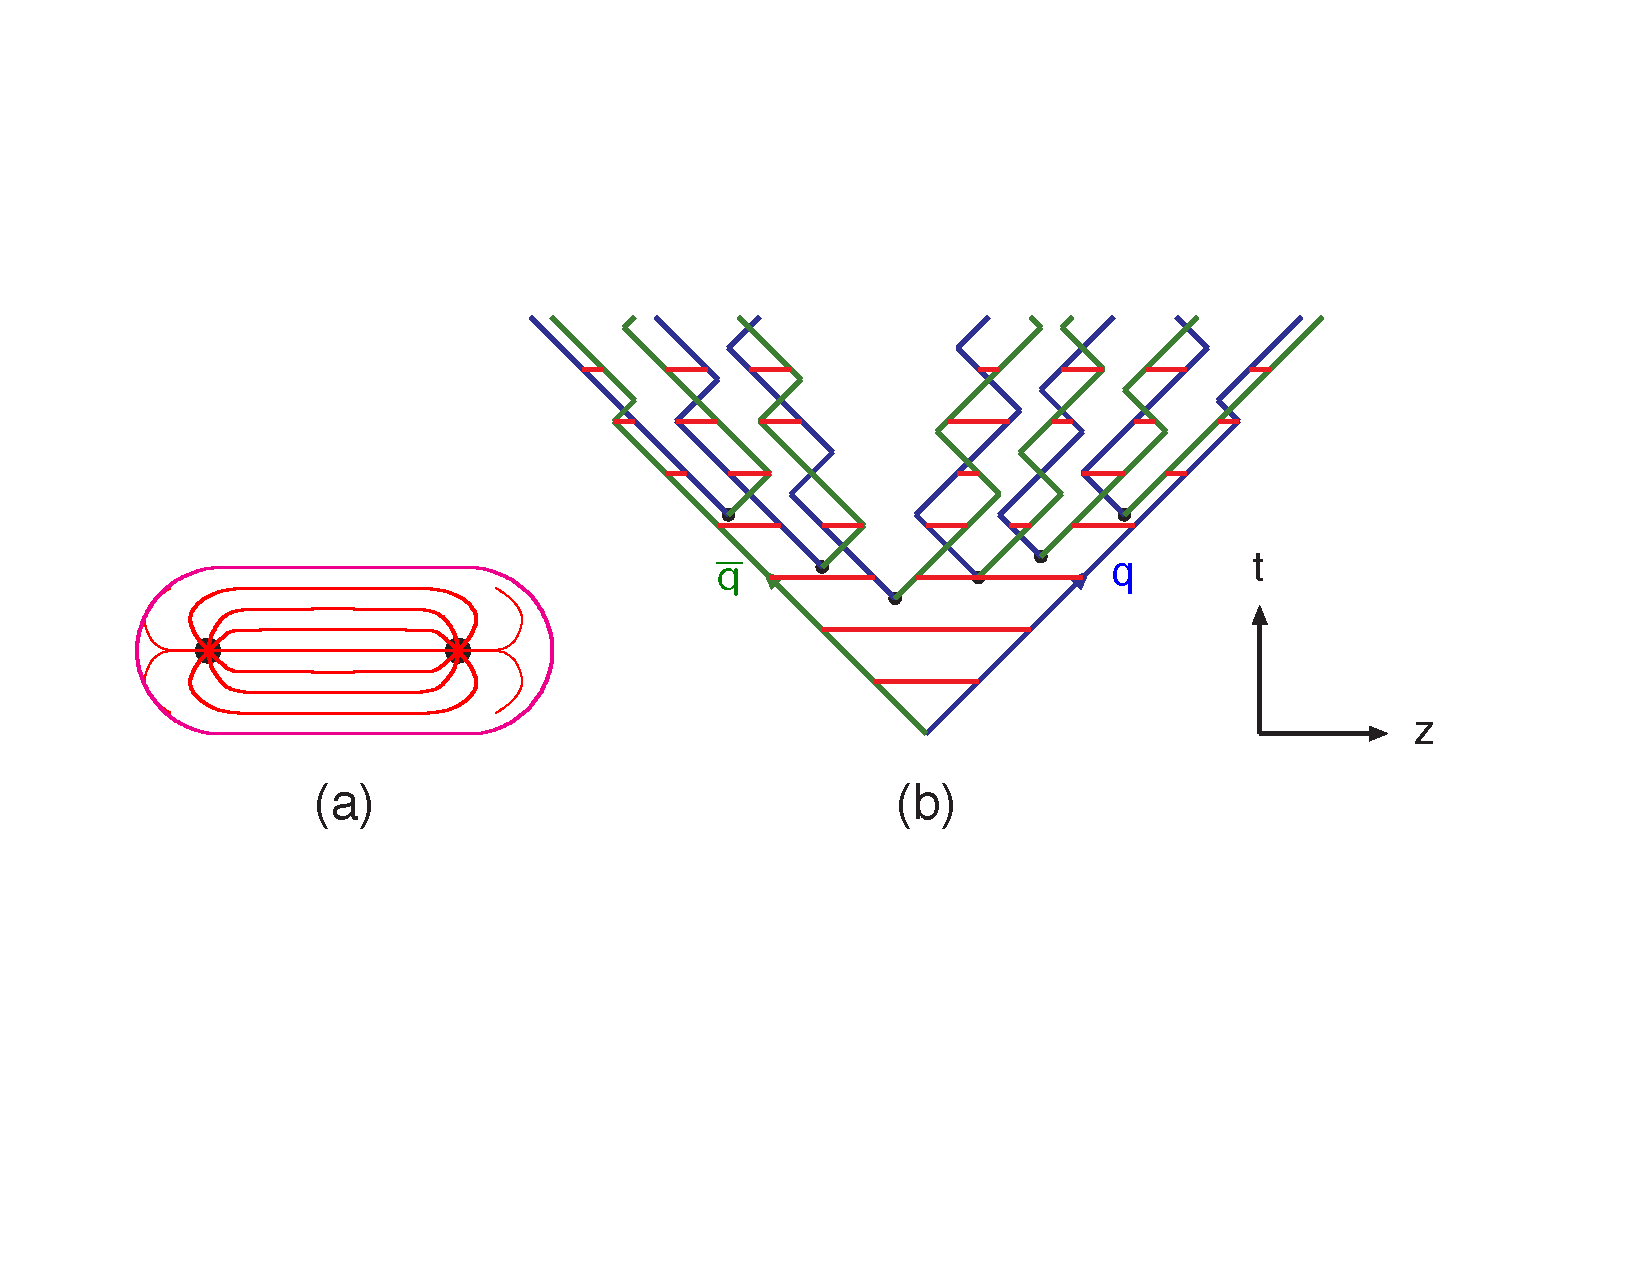
\includegraphics[width=0.75\textwidth]{pics/stringone.pdf}
\caption[]{ (a) A flux tube spanned between a quark and an antiquark. (b) The motion
and breakup of a string system, with the two transverse degrees of freedom suppressed
(diagonal lines are (anti)quarks, horizontal ones snapshots of the string field).
\cite{eventGenerators} }
\label{fig:fluxtube}
\end{figure}

\subsubsection*{Cluster model}
Instead of a string model HERWIG~\cite{} uses a cluster model~\cite{herwigManual} for hadronisation. The advantage of cluster models is that they require a smaller number of parameters than string models. The model is based on the preconfinement property of parton showers, i.e. the colour structure of the shower at any evolution scale $Q_0$ is such that colour singlet combinations of partons can be formed with an asymptotically 
universal invariant mass distribution. The invariant mass does not depend on the initial hard process scale $Q$, but only on $Q_0$ and the QCD scale $\Lambda _ \mathrm{QCD}$, when $Q \gg Q_0$.

The cluster model starts from transforming all gluons non-perturbatively into $\mathrm{q \bar q}$ pairs, which requires that the gluons get a mass, which must be at least twice the lightest quark mass. After the gluons are transformed into quarks, the adjacent colour lines can be clustered together to colour singlet states with mesonic quantum numbers. The momentum of these clusters is defined to be the sum of the momenta of the clustering partons. According to preconfinement, the mass distribution of these clusters is independent of the details of the hard scattering. Additionally the clusters can be regarded as highly excited hadron resonances and decayed into the final state hadrons.

Some of these initial clusters are too heavy to reasonably describe an excited state of a hadron. These must be
split before they are allowed to decay. The cluster $C$ is split if its mass fulfils the condition~\cite{}

\begin{equation}
M_C^p \geq M_\mathrm{max}^p  + \left( m_1 + m_2\right)^p,
\label{eq:clustermass}
\end{equation}

\noindent where $m_{1,2}$ are the masses of the constituents partons of the cluster and $M_\mathrm{max}$ and $p$ are the main parameters of the model. These have to be chosen separately for clusters containing light, charmed and bottom quarks. When a cluster is split, a pair of light quarks is generated from the vacuum and two new clusters are made, both containing one quark from the original cluster and one from the newly generated pair. The splitting is continued until no clusters with masses $M_C$ fulfilling the equation ~\ref{eq:clustermass} remains.

\begin{figure}
\centering
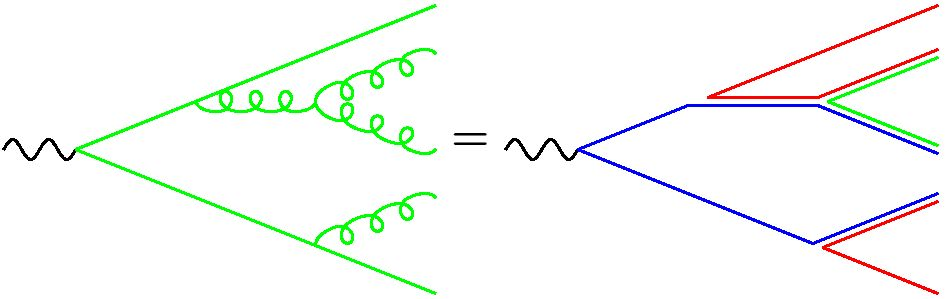
\includegraphics[width=0.75\textwidth]{pics/planar.jpg}
\caption[]{ Colour structure of a parton shower to leading order in Nc.
\cite{eventGenerators} }
\label{fig:colourstructure}
\end{figure}

When the clusters are light enough, they decay into final state hadrons. If the mass of the cluster is high enough for decaying into a baryon-antibaryon pair, there is a parameter deciding whether the cluster undergoes mesonic or baryonic decay. For a mesonic decay a quark-antiquark pair is created from the vacuum and for the baryonic decay a diquark-antidiquark pair is made. Then the exact decay products are chosen and the cluster decays isotropically in the rest frame of the cluster. If there are partons produced in the perturbative phase involved in the decay, they retain their original direction in the cluster rest frame, up to some Gaussian smearing. If the cluster mass is too low to decay into a pair of mesons, it decays into the lightest possible hadron and some energy and momentum is exchanged with the adjacent clusters. At the end we are left with the final state hadrons, some of which might still decay until the end of the simulation if they are very short-lived.~\cite{} 

\subsubsection{Jet energy loss}
\subsubsection*{Discovery of jet quenching via leading hadron suppression}
First evidence of jet quenching comes from observing high $\pt{}$ tracks, i.e. the leading hadrons.


Jet quenching in heavy-ion collisions is usually quantized with the nuclear modification factor $R_{AA}$, which is  is defined as
%the yield in heavy-ion collisions divided by the yield in proton-proton collisions and scaled by the The nuclear modification factor

\begin{equation}
R_{AA}\left(\pt{}\right) = \frac{(1/N_{AA}^{evt})\dd {N^{AA}}/\dd {\pt{}}}{\left< N_{coll}\right> (1/N_{pp}^{evt})\dd {N^{pp}}/\dd {\pt{}}}\label{eq:raa}
\end{equation}
\noindent where $\dd{N^{AA}}/\dd{\pt{}}$ and $\dd{N^{pp}}/\dd{\pt{}}$ are the yields in heavy-ion and proton-proton collisions, respectively and $\left< N_{coll}\right>$ is the average number of binary nucleon-nucleon collisions in one heavy-ion event. The number of binary collisions can be calculated from the Glauber model as shown in Sec.~\ref{sec:glauber}. From the point of view of direct production a heavy-ion collision can be estimated relatively well to be only a series of proton-proton collisions. 

If the medium has no effect on high $\pt{}$ particles the nuclear modification factor should be 1. At RHIC and LHC this has been observed to be as low as 0.2 because of jet quenching. Measurements of $R_{AA}$ from different sources are shown in Fig.~\ref{fig:Raa}

\begin{figure}[hbt]
	\centering
                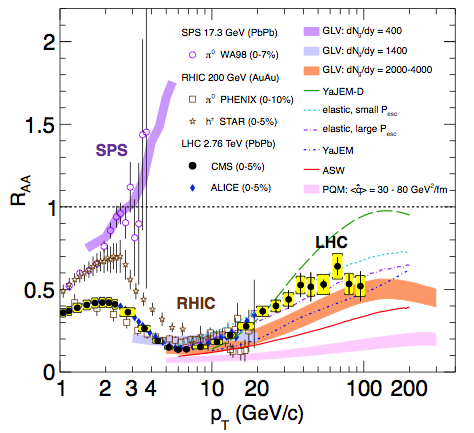
\includegraphics[width=0.65\textwidth]{pics/Raaplot}
        \caption[Measurements of the nuclear modification factor $R_{AA}$ in central heavy-ion collisions]{Measurements of the nuclear modification factor $R_{AA}$ in central heavy-ion collisions at three different center-of-mass energies, as a function of $\pt{}$, for neutral pions ($\pi^0$), charged hadrons ($h\pm$), and charged particles~\cite{Aamodt:2010jd, Aggarwal:2001gn, d'Enterria:2004ig, Adare:2008qa, Adams:2003kv}, compared to several theoretical predictions~\cite{Dainese:2004te, Vitev:2002pf, Vitev:2004bh, Salgado:2003gb, Armesto:2005iq, Renk:2011gj}. The error bars on the points are the statistical uncertainties, and the yellow boxes around the CMS points are the systematic uncertainties. The bands for several of the theoretical calculations represent their uncertainties~\cite{CMS:2012aa}.}
        \label{fig:Raa}
\end{figure}


The nuclear modification factor can also be used to quantify anisotropy. In the study of anisotropy $R_{AA}$ in-plane and out-of-plane can be compared. The distance traveled through medium is largest out-of-plane which leads to stronger suppression in this direction. The nuclear modification factor as a function of $\Delta\phi=\phi-\psi_n$ is given by

\begin{eqnarray}
R_{AA}\left(\Delta\phi, \pt{}\right) &=& \frac{(1/N_{AA}^{evt})\dd {^2N}^{AA}/d\Delta\phi \dd {\pt{}}}{\left< N_{coll}\right> (1/N_{pp}^{evt})\dd {N^{pp}}/\dd {\pt{}}} \approx \frac{\dd {N^{AA}}/\dd {\pt{}}\left( 1+2\cdot v_2\cos{(2\Delta\phi)} \right)}{\left< N_{coll}\right> \dd {N^{pp}}/\dd {\pt{}}} \nonumber \\ &&\nonumber\\
&=& R_{AA}^{incl}(\pt{}) \left( 1+2\cdot v_2\cos{(2\Delta\phi)} \right).
\label{eq:raaandv2}
\end{eqnarray}	

The yield of proton-proton collisions is independent of the reaction plane and the yield in heavy-ion collisions is modulated by the second harmonics. In Eq. (\ref{eq:raaandv2}) $R_{AA}$ is approximated only up to the second harmonics.
From \eq{eq:raaandv2} it follows that

\begin{equation}
\frac{R_{AA}\left(0, \pt{}\right)-R_{AA}\left(\pi/2, \pt{}\right)}{R_{AA}^{incl}(\pt{})} \approx \frac{R_{AA}^{incl}(\pt{}) \left(1+2 \cdot v_2-(1-2 \cdot v_2) \right)}{R_{AA}^{incl}(\pt{})} = 4 \cdot v_2
\label{eq:raaandv2result}
\end{equation} 
%At high-$\pt{}$, the pQCD processes are dominant, hence the $v_n$ (or $R_{AA}(\Delta\phi, \pt{})$) characterize the path length-dependence of the energy loss process. 
The observed $R_{AA}\left(\Delta\phi, \pt{}\right)$  from PHENIX measurements in Au-Au collisions at $\sqrt{s}=200\gev$~\cite{PhysRevC.80.054907} is compared to $R_{AA}$ using $v_2$  via \eq{eq:raaandv2} in Fig.~\ref{fig:RAAv2}. They agree very well within the statistical errors for all centrality and $\pt{}$ bins.
\begin{figure}[htb]
	\centering
                \includegraphics[width=0.5\textwidth]{pics/RAAandv2Correlation}
        \caption[A comparison between observed $R_{AA}\left(\Delta\phi, \pt{}\right) $ and $R_{AA}$ using $v_2$]{ A comparison between observed $R_{AA}\left(\Delta\phi, \pt{}\right) $ and $R_{AA}$ using $v_2$ from PHENIX measurements of Au-Au collisions at $\sqrt{s}=200\gev$. On the X-axis is the measured $R_{AA}\left(\Delta\phi,\pt{}\right)$. On the y-axis is the inclusive $R_{AA}$ multiplied by  $1+2v_2\cos\left(\Delta\phi\right)$~\cite{PhysRevC.80.054907}.}
        \label{fig:RAAv2}
\end{figure}

At high-$\pt{}$, the pQCD processes are dominant, hence the $v_n$ (or $R_{AA}(\Delta\phi, \pt{})$) characterize the pathlength-dependence of the energy loss process.

Jet quenching is not the only high $\pt{}$ phenomenon studied in heavy-ion collisions. Another property is jet fragmentation. The high momentum parton created in the initial collision fragments into a number of partons with smaller $\pt{}$. Jet fragmentation occurs also in proton-proton collisions in the vacuum, but it can be modified due to the presence of the medium. In order to study the jet fragmentation function ($D(z)$, where $z= \pt{}^h/\pt{}^{part}$) modification due the medium, we use the two-particle correlations. The particle yield can be extracted from the correlation function. The background from the flow processes is correlated and needs to be subtracted to get the particle yield associated only with the jet. The ratio of the jet yields in Au-Au and p-p collision $I_{AA} = {Y^{Au+Au}}/{Y^{p+p}}$ characterizes the jet fragmentation modification \cite{Aamodt:2011vg}. $I_{AA}$ probes the interplay between the parton production spectrum, the relative importance of quark-quark, gluon-gluon and quark-gluon final states, and energy loss in the medium.


\begin{figure}[ht]
\centering
\includegraphics[width=0.9\textwidth]{pics/highptv2}
\caption[Elliptic flow, $v_2$ from $\pt{}=1$ to $60\gevc$]{ Elliptic flow, $v_2$, as a function of the charged particle transverse momentum from $1$ to $60\gevc$ with $\left|\eta\right|<1$ for six centrality ranges in Pb-Pb collisions at $\snn=2.76\tev$, measured by the CMS experiment.~\cite{Chatrchyan:2012xq}. }
\label{fig:highpt}
\end{figure}

\subsubsection*{Theory of jet quenching}



High momentum particles are very rare and they are only produced in the initial collisions. After they are created they escape the medium before a thermal equilibrium is reached. Thus they are not part of the pressure-driven collective expansion. Instead high momentum yield is suppressed because of energy loss in the medium. When propagating through the medium these partons lose energy as they pass through the medium. This is referred to as jet quenching. Jet quenching depends on the path lengths through the medium. Thus anisotropy in this region is mainly dependent on the collision geometry and density of medium.


The energy loss of partons in medium is mainly due to QCD bremsstrahlung and to elastic scatterings between the parton and the medium. 


The radiative energy loss mechanism is given in terms of the transport coefficient $\left<\hat q\right>$, which describes the average momentum transfer between the medium and parton~\cite{jetBroadeningPpb1}. The exact definition of this depends on the theoretical formalism used to describe the energy loss mechanism. 

Many of the energy loss models exploit the analogy between the QCD interaction of parton propagating through the colored medium and the QED energy loss of electron propagating through material. An electron propagating through matter loses its energy by photon Bremsstrahlung radiation. In the simplest case, each individual scattering center results in a single emission of a photon. This is known as the Bethe-Heitler regime~\cite{BetheHeitler}. The energy spectrum of radiated photons $\nicefrac{dN}{dE}$ is, in this case, proportional to $\nicefrac{1}{E}$. However, the Bremsstrahlung photon, can be radiated only when the distance between the scattering centers is larger than the formation length. In the limit, when the scattering centers are closer than the formation length, the Bremsstrahlung process is suppressed. This phenomenon is known as the Landau-Pomeranchuk-Migdal (LPM)~\cite{Landau:1953um,Migdal:1956tc} suppression. The radiated spectrum in this regime is proportional to $\nicefrac{1}{\sqrt{E}}$.

Lower energy photons are further suppressed by the destructive interference leading to the suppression of Bremsstrahlung photons of $E < \gamma \omega_p$, where $\omega_p$ is the plasma frequency of the radiator. This is knows as Dielectric suppression. The photon energy distribution in this regime is proportional to the energy of the photon. A schematic view of the effect of these three regimes is shown in Fig.~\ref{fig:bremsstrahlung}.

\begin{figure}
\centering
\includegraphics[width=0.9\textwidth]{pics/BremsstrahlungElectron}
\caption[Photon spectrum]{ The expected bremsstrahlung spectrum for a electron propagating through material.  ~\cite{Bosted1993QuantummechanicalSO}. }
\label{fig:bremsstrahlung}
\end{figure}

The simplest energy loss process is elastic QCD scattering off the medium partons. In elastic scatterings the recoil energy of the scattered partons are absorbed by the thermal medium, which reduces the energy of the initial parton. The mean energy loss from elastic scatterings can be estimated by

\begin{equation}
\left<\Delta E\right>_{\mathrm{el}}=\sigma \rho L \left<E\right>_{\mathrm{1\,scatt}}\propto L,
\label{eq:elastic}
\end{equation}

\noindent where $\sigma$ is the interaction cross section and $\left<E\right>_{1 scatt}$ is the mean energy transfer of one individual scattering~\cite{Majumder:2010qh}. This assumption holds if the mean energy is independent of the total energy of the parton ($E$). The transport coefficient of elastic scattering, $\left< \hat q_\mathrm{el}\right> = \nicefrac{\left< \Delta E\right>}{L}$, is defined as the mean energy los per unit path length.

Another energy loss mechanism is medium-induced radiation. In QCD this radiation is mainly due to the elementary splitting processes, $q\rightarrow qg_r$ and $g\rightarrow gg_r$. Assuming that the parton is moving with the speed of light radiation energy loss can be estimated by

\begin{equation}
\left<\Delta E\right>_{rad}\propto T^3L^2,
\label{eq:radiative}
\end{equation}

\noindent where $L$ is the length of the medium and $T$ is its temperature~\cite{Dominguez:2008vd}. The different exponents of $L$ in equations \ref{eq:elastic} and \ref{eq:radiative} indicate that radiative energy loss is dominant over elastic energy loss.


There are several models that attempt to describe the nature of the energy loss mechanism. The most used models can be divided into four formalisms.
%
%\begin{itemize}
%\item Thermal effective theory formulation (AMY)~\cite{Arnold:2001ms, Arnold:2002ja}
%\item Opacity Expansion ((D)GLV/WHDG and ASW-SH)~\cite{Salgado:2003gb, Gyulassy:2000er, Gyulassy:1999zd, Wiedemann:2000za} 
%\item Higher Twist approach~\cite{Wang:2001ifa, Majumder:2009zu} 
%\item Multiple soft scattering approximation BDMPS-Z (ASW-MS)~\cite{Baier:1996kr, Zakharov:1996fv, Baier:1998kq, Salgado:2003gb}
%\end{itemize}

In the Gyulassy-Levai-Vitev (GLV)~\cite{Gyulassy:1999zd} opacity expansion model
 the radiative energy loss is consiered on a few scattering centers $N_{scatt}$. The radiated gluon is constructed by pQCD calculation as summing up the relevant scattering amplitudes in terms of the number of scatterings. Another approach into opacity expansion is the ASW model by Armesto, Salgado and Wiedermann~\cite{Wiedemann:2000za}.

Thermal effective theory formulation by Arnold, Moore and Yaffe (AMY)~\cite{Arnold:2001ms} uses dynamical scattering centers. It is based on leading order pQCD hard thermal loop effective field theory. This model assumes that because of the high temperature of the plasma the strong coupling constant can be treated as small. The parton propagating through the medium will lose energy from soft scatterings and hard scatterings.

The above models calculate the energy loss while the parton propagates through the medium, focusing on the pQCD part. The higher twist (HT) approach by Wang and Guo~\cite{Wang:2001ifa} implements the energy loss mechanism in the energy scale evolution of the fragmentation functions.

The last category is formed by the Monte Carlo methods. The PYTHIA event generator~\cite{pythia} is widely used in high-energy particle physics. Two Monte Carlo models based on PYTHIA describing the energy loss mechanism are PYQUEN~\cite{Lokhtin:2005px} and Q-Pythia~\cite{Armesto:2009zc}. Other Monte Carlo models include JEWEL~\cite{Zapp:2008gi} and YaJEM~\cite{Renk:2009nz}.



\subsubsection{New paradigm of jet Quenching}
As described in the previous section there have been many experimental evidences of jet energy loss, such as the suppression of inclusive hadron spectra at high transverse momentum~\cite{Adcox:2001jp,Adams:2003im,Arsene:2003yk,Khachatryan:2016odn,Acharya:2018qsh}, the modification of back-to-back hadron-hadron~\cite{Adare:2007vu,Aamodt:2011vg} and direct photon-jet correlations~\cite{Adare:2012qi}, and the modification of reconstructed jet spectra~\cite{Adam:2015ewa} and jet substructure~\cite{Sirunyan:2018qec,Chatrchyan:2014ava,Acharya:2018uvf}, as compared to the expectations from elementary proton-proton collisions.


The first indications of jet quenching, such as $R_{\mathrm{AA}}$, looked essentially at the leading hadrons of jets, the hard part, ignoring the soft scale part of jet phenomena. However, experimental methods have since improved; jet reconstruction algorithms have become reliable in the LHC era. Instead of the leading hadron we can study the entire jet shower. 

-Jet RAA
-Jetscape

Thus the new paradigm in jet quenching in heavy-ion collisions involves multi-scale problems~\cite{Kurkela:2014tla,Tachibana:2018yae}. The elementary scattering and the subsequent branching process down to non-perturbative scales are dominated by hard scales in the vacuum as well as in the medium. Soft scales, of the order of the temperature of the medium, characterise the interactions of soft partons produced in the shower with the QGP. Soft scales also rule hadronisation, which is expected to take place in vacuum for sufficiently energetic probes, even though some modifications can persist from modifications of color flow~\cite{Aurenche:2011rd,Beraudo:2011bh,Beraudo:2012bq}. Understanding the contributions from the different processes to the jet shower evolution in medium and their scale dependence is crucial to to constrain the dynamics of jet energy loss in the expending medium, the role of colour coherence~\cite{CasalderreySolana:2012ef}, and fundamental medium properties like temperature dependent transport coefficient~\cite{DEramo:2012uzl,Ayala:2016pvm}.


\subsubsection*{Lund diagram}

\begin{figure}
\centering
\includegraphics[width=0.75\textwidth]{figures/regions4.eps}
\caption[]{Parametrically accurate picture of how a medium-modified parton cascade fills the phase space. At time $t$, quanta can be formed up to momentum scale $k_{\rm form}$ and they are formed with $O(1)$ probability per $\log p$ at lower scale $k_{\rm split}$. Quanta below $k_{\rm split}$ split further and their energy cascades to the thermal scale $T$ in less than an epoch $t$. Transverse Brownian motion moves quanta up to the angle $\theta_{\rm BR}(p)$ denoted by the thick purple line.  The Moli\`ere region at larger $\theta$ is dominated by rare large angle scattering. At even larger angle, there are $O(\alpha_s)$ quanta per double logarithmic phase space  from DGLAP 'vacuum' radiation, and for momenta below $k_{\rm split}$ these cascade within time $t$ to $T$. After the jet escapes the medium, the jet and the emitted fragments will undergo vacuum radiation. This late time vacuum radiation emitted by the original parton dominates at sufficiently small $\log \theta$  (regions marked ``late DGLAP'' and bounded by $\theta_{\rm vac}$ and $\theta_\alpha$),  whereas the late time radiation of the fragments dominates in the region  denoted by ``Vacuum cascade of the medium induced quanta''. ~\cite{Kurkela:2014tla}. }
\label{fig:cascades}
\end{figure}

The different momentum and angular scales are subject to different physical phenomena. Figure~\ref{fig:cascades} shows the relevant medium modification phenomena for different regions of the phase space at time $t$, when a jet propagates through a thermal cloud of temperature $T$. As in a practice jets propagate over a finite path-length $L$ in QCD matter, Fig.~\ref{fig:cascades} can be taken as a representation of the distribution of partonic jet fragments at moment $t \approx L$, when the jet escapes the medium.

The region marked as DGLAP is dominated by the primary vacuum splittings. This region is determined by $\theta > \theta_\mathrm{vac}$ with

\begin{equation}
\theta_\mathrm{vac} \propto \nicefrac{1}{\sqrt{pt}}.
\end{equation}


Medium-induced parton branching fills the $\log p$-$\log$-$\theta$-plane from the bottom up (in $p$) and from the inside out (in $\theta$). This is because transverse momentum is acquired by Brownian motion in the medium, $k_\perp^2 \propto \hat q t$. Then the formation time constaint $t \geq \nicefrac{p}{k_\perp^2} \approx \nicefrac{p}{\hat q t}$ implies that medium-induced quanta can be formed in the region $p \leq k_\mathrm{form}$ where

$$k_\mathrm{form}\left(t\right) = \hat q t^2$$.

The probability of finding a splittee with a momentum $p$ with $p < k_\mathrm{form}$ is 

\begin{equation}
\frac{\mathrm d P_\mathrm{find}\left(t\right)}{\mathrm d \log p} \propto \alpha_s \nicefrac{t}{t_\mathrm{form}}\left(p\right) \propto \alpha_s \hat q ^{nicefrac{1}{2}} p^{-\nicefrac{1}{2}} t
\end{equation} 

Not all quanta will stay where they were created. Those modes that have time to lose a significant fraction of their energy will cascade to a significantly lower scale $p$. For LPM-type radiation, the splitting that degrades energy the most is the hardest splitting. 

The $\log p $ distribution has the same $\frac{1}{\sqrt{p}}$ dependence as in the LPM region

\begin{equation}
\frac{\mathrm{d}n}{\mathrm{d}\log p} = \frac{1}{p}\frac{\mathrm{d}\epsilon}{\mathrm{d}\log p} \approx \alpha_s \frac{\sqrt{\hat q t}}{\sqrt{p}}
\end{equation}

Also the quanta originating from the DGLAP region will undergo medium interactions that will make the quanta radiate and split. The distribution of radiation is the same as from any other mode. Above a certain momentum scale $k_\mathrm{split}$ the distribution of originating daughters is 


\begin{equation}
\frac{\mathrm d P_\mathrm{find}}{\mathrm d \log p \mathrm{d} \log \theta} \approx \alpha_s \frac{t}{t_\mathrm{split}\left(p\right)},
\end{equation} 

Note that the ratio $\nicefrac{t}{t_\mathrm{split}}$ is smaller than 1 for nodes above $k_\mathrm{split}$ and therefore the number of daughters is smaller than the number of vacuum splitted quanta. Below $k_\mathrm{split}$ the cascade is similar to the medium cascade and the number of quanta become

\begin{equation}
\frac{\mathrm{d}n}{\mathrm{d}\log p \mathrm{d} \log \theta} \approx \alpha_s \frac{t}{t_\mathrm{split}\left(p\right)}, \text{ for } p < k_\mathrm{split}\left(p\right)
\end{equation}


The angular distribution is driven by two mechanisms; Multiple soft scatterings give rise to transverse Brownian motion, which determines the distribution at small angles. The typical angle reached in the LPM region is 

\begin{equation}
\theta_\mathrm{BR}\left(p\right) \approx \frac{\sqrt{\hat q t}}{p}, \text{ for } k_\mathrm{form} > p > k_\mathrm{split},
\end{equation}

while in the medium cascade region of the phase space this becomes

\begin{equation}
\theta_\mathrm{BR}\left(p\right) \approx \left(\frac{T}{p}\right)^{\frac{3}{4}}
\end{equation}

Large angular scales cannot be reached by Brownian motion, but can arise from rare large angle scatterings, described by Molière~\cite{}.


\subsubsection{Jet shape measurements}


%\subsubsection*{DGLAP}
%
%Quantum mechanical formation time prevents emission faster than a time it takes to separate the wave packets of the splitter and the splittee. In general, splittees at a scale $p < Q$ can form at a time $t  \geq \nicefrac{p}{k_\perp^2}$ set by their inverse transverse energy. For jet evolution in the vacuum the angular distribution is determined by the primary decay kinematics of the splittee, $t \geq \nicefrac{p}{k_\perp^2} \approx \nicefrac{1}{p \theta^2}$. Therefore, the logarithmically ordered DGLAP 'vacuum' parton shower fills the $\log p$-$\log\theta$-plane from the outside in. In the entire region determined by $\theta > \theta_\mathrm{vac}$ with
%
%\begin{equation}
%\theta_\mathrm{vac} \propto \nicefrac{1}{\sqrt{pt}},
%\end{equation}
%
%one finds with a probability $O\left(\alpha_s\right)$ per logarithmic phase space quanta due to vacuum radiation, 
%
%\begin{equation}
%\frac{\mathrm{d} P_\mathrm{find}}{\mathrm{d} \log p \mathrm{d}\log \theta} \propto \alpha_s
%\end{equation}
%
%The region where this primary splitting gives the dominant contribution in the $\log p$-$\log \theta$-plane is marked as DGLAP in Fig.~\ref{fig:cascades}.
%
%\subsubsection*{LPM}
%
%
%
%\subsubsection*{Medium cascade}







\subsection{QGP in Small systems}
After the existence of QGP in heavy-ion collisions has been established, attention has been turned to small systems. Proton-proton (pp) and proton-Lead (pPb) collisions have been studied at LHC and RHIC has studied a host of different collision systems; namely proton-Gold (pAu), deuteron-Gold (dAu) and Helium$^3$-Gold (He$^3$Au) collisions starting in 2000. %At LHC small systems have been studied in proton-Lead (pPb) collisions. First observations seemed to indicate that the signals taken to confirm the existence of QGP in heavy-ion collisions disappear in these small systems.

Already before the era of modern colliders, collective behaviour in proton-proton collisions was considered by names like Heisenberg, Fermi and Bjorken.~\cite{Nagle:2018nvi} Eventually there were some experimental searches of QGP in pp and $p\bar p$ collisions in E735 at Tevatron~\cite{Alexopoulos:1993wt} and MiniMAX~\cite{Brooks:1999xy}. However no conclusive evidence was found. 

In the early years of RHIC these small systems were mostly considered as control measurement, for example in constraining nuclear modified parton distribution functions (nPDFs) that determine the initial gluon distributions that determine the first epoch
of heavy-ion collisions~\cite{Shen:2015qta, Adare:2015lcd}. 

In 2010 ultrahigh-multiplicity pp collisions were studied at CMS. The study found that particles had a weak but clear preference to be emitted along a common transverse $\phi$ angle across all rapidities ~\cite{Salgado:2016jws}. This seemed like behaviour were similar to AA collisions, but it was argued that it could as well come from momentum correlations present in the earliest moments of the collision.

In 2012 LHC ran its first pPb data taking period. Around the same time dAu data was reexamined at RHIC. Now it was revealed that most of the flow signatures attributed to hydrodynamic expansion in AA collisions also existed in smaller systems.
\begin{figure}[b!]
\centering
            	\includegraphics[height=2.4in]{pics/figure_phenix_geometry_new}
                \caption{Calculations of the intial energy density in small collision systems at RHIC and the resulting hydrodynamic evolution.}
	\label{fig:smallsystems1}
\end{figure}



-Sub nucleonic structure needed to describe intial conditions in pA, pp
\subsubsection{Collective phenomena}
The most rugged analysis of collective behaviour concerns the two (or more) particle correlations, often parametrised via the relative azimuthal angle and pseudorapidity differences, $\Delta \phi$ and $\Delta \eta$ respectively. Figure ~\ref{fig:smallsystems2} shows two-particle correlations measurements in PbPb, pPb and pp collisions at the LHC. In PbPb collisions long-range correlations dominate over short-range phenomena. This shows in the two ridges at $\Delta \phi = 0 $ and $\Delta \phi = \pi$. At $\Delta\phi\approx\Delta\eta\approx0$, there is a peak coming from single jet fragmentation. Since the away-side jet can be spread out in $\Delta\eta$, this contribution disappears when compared to the flow contribution at the away side ridge. In pPb, and pp the near side peak is more distinguished and the away-side jet contribution starts to show. Still, one can see long-range correlations that seem like flow-like collective behaviour in both systems. 
\begin{figure}[b!]
\centering
            	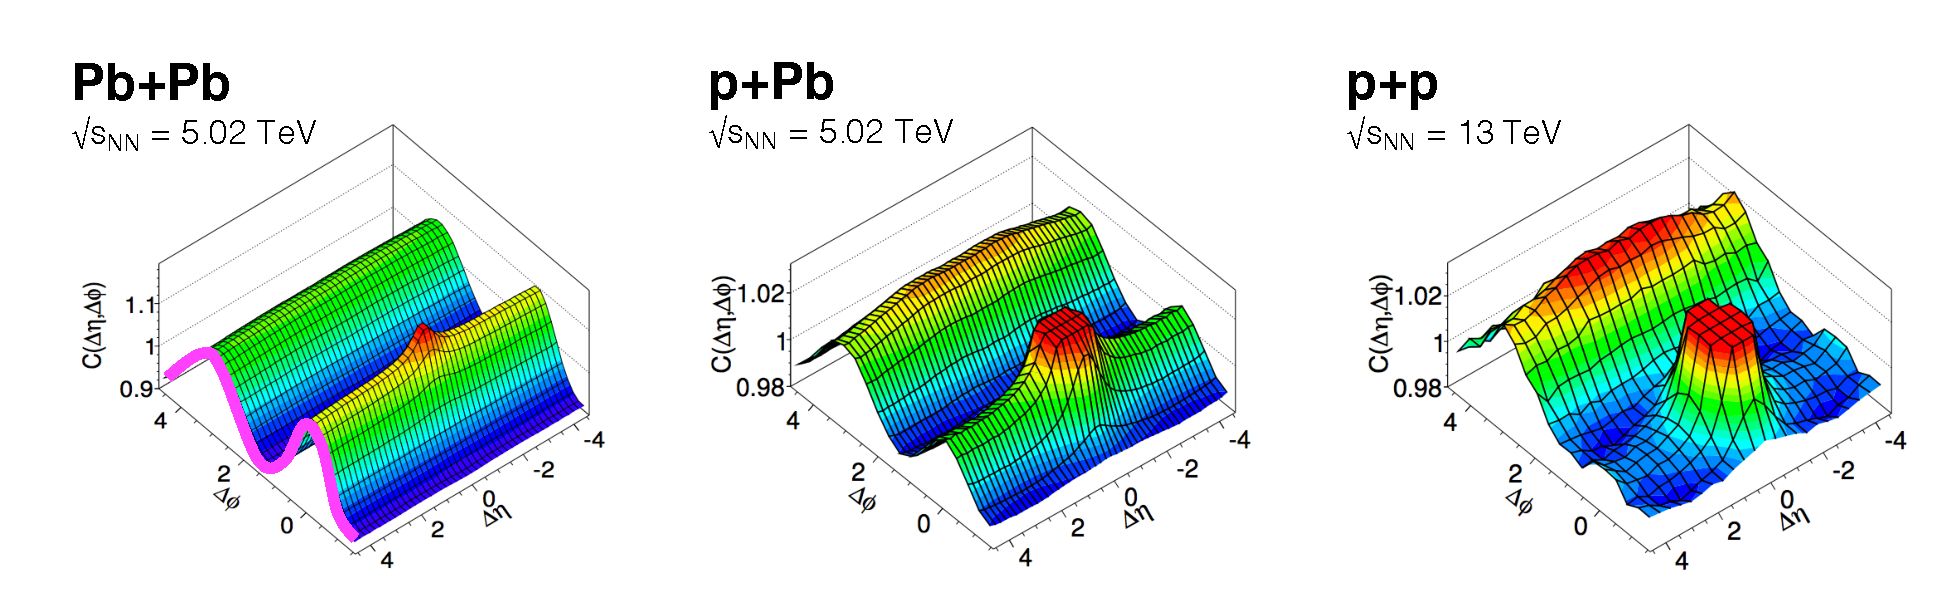
\includegraphics[width=0.9\textwidth]{pics/figure_ridges}
                \caption{Two-particle correlation results in PbPb, pPb, and pp collisions at the LHC~\cite{}. }
	\label{fig:smallsystems2}
\end{figure}

In addition to the two particle correlations, correlations have been observed in the form of $v_n$ coefficients both at LHC and at RHIC. The results have also been described  with hydrodynamical models, although the applicability of said models is questionable, because of the large Reynolds numbers in small systems. Figure \ref{fig:smallsystems1} shows results for $v_2$ in different collisions systems at RHIC as measured by PHENIX. These different systems provide also different initial geometries. dAu collisions naturally have an ellipsoidal form, while a He3 collision has a triangular form and thus produces larger triangular flow, $v_3$ components. 

Other observations that produce flow-like results include mass ordered $v_2$ coefficients and higher order harmonics coming from fluctuations in the initial geometry. Thus all the major collective flow phenomena observed in heavy-ion collisions have been also identified in small systems.

One open question is identifying the point the point, where flow-like correlations end. The question has proved challenging since low multiplicity events are dominated by non-flow phenomena. This makes observations in low multiplicity events model/method dependant. Different methods assess non-flow contributions differently. Thus some methods fail to observe a signal in cases, where others do and it is unclear whether this is true collective motion or it comes from non-flow contributions.

\subsubsection{Absence of jet quenching}
In A+A collisions, an important confirmation of the standard model comes from the energy loss of high $\pt{}$ partons traversing the medium, referred to as jet quenching~\cite{Gyulassy:2003mc,doi:10.1146,Accardi:2009qv}. In 2003 the jet quenching effect was observed to disappear in d+Au collisions. This was taken as an indication that no QGP was created. Similarly at LHC no jet modification has been observed in pPb collisions. Fig. \ref{fig:smallsystems3} shows the nuclear modification factor $R_{\mathrm{pA}}$ in pPb collisions as measured at the LHC. 

The lack of jet modification seems surprising considering the multitude of flow observations supporting the existence of QGP in small systems. One possible explanation is simply the size of medium. In PbPb collision partons traversing through the medium lose energy to the medium. If the medium is very small there is limited time for interaction with the medium. 

Calculations indicate that there should be modification in the most central pPb collisions, but selecting these in the analysis is complicated. In PbPb collisions most of the particle production comes from the medium and thus the total multiplicity is a good indicator of centrality. In pPb collisions, however the total multiplicity is smaller and is more strongly influenced by jet phenomena. Events with jets have naturally larger multiplicities and are more likely to be classified as central events.

So far the only observable indicative of jet quenching in pPb collisions is the high $\pt{}$ $v_2$. In heavy-ion collisions this is not explained by hydrodynamics. Instead it is assumed to come from jet quenching with different path lengths through the medium in different directions. In Fig.\ref{fig:smallsystems3} ATLAS and CMS measurements of $v_2$ in pPb and PbPb collisions are shown. The pPb results seem to follow a very similar pattern. 


\begin{figure}[b!]
\centering
            	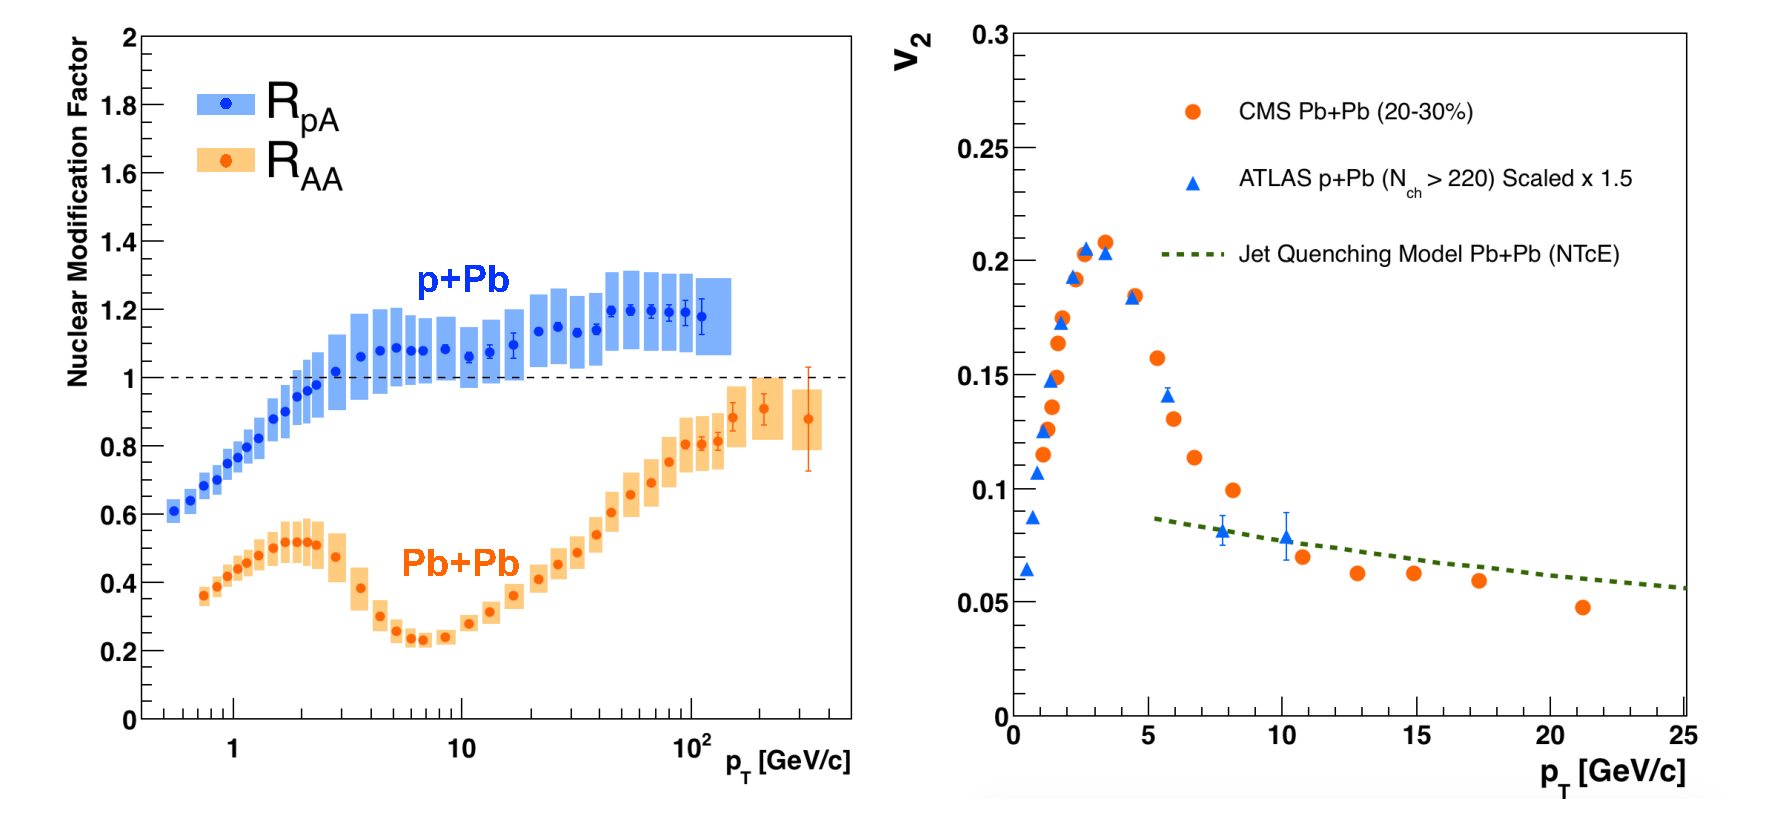
\includegraphics[width=0.9\textwidth]{pics/figure_ppb_jetquenching.pdf}
                \caption{RpA in proton-lead collisions}
	\label{fig:smallsystems3}
\end{figure}


\begin{table}[htb]
\centering
\caption{Summary of observations in small system}
\label{tab:Smallsystem}
\begin{tabular}{ l | c | c | r }
  Observable & PbPb & pPb & pp \\
    \hline			
  Jet RpA/RAA & Modified & No modification &  - \\
  Hadron RpA/RAA & Modified & No modification &  -\\
  Heavy flavors & & & \\
 % Jet quenching & Observed & No  \\
  Jet shape & Broadening & No observations & - \\
  Two-particle correlations & Ridge & Ridge & Ridge  \\
  $v_2$ & Observed & Observed & Observed \\
  Mass ordered flow & & & \\
  Higher ordered harmonics & &  &\\
  High $\pt{}$ $v_2$ & Observed & Maybe & - \\
  \hline
  \end{tabular}
  \end{table}

\subsubsection{Centrality determination in small systems}
\label{sec:smallsystemcentrality}
In lead-lead collisions the total multiplicity of the event is a good indicator of the centrality of the collision. In proton-lead collisions the connection of multiplicity and centrality is less clear. In \pPb collisions the impact parameter is only loosely correlated to $N_\mathrm{part}$ or $N_\mathrm{coll}$. Hence, although one uses traditionally the term centrality to refer to these measurements, the relevant parameters are $N_\mathrm{part}$ and $N_\mathrm{coll}$~\cite{Adam:2014qja}.

The Glauber model~\cite{Miller:2007ri} is generally used to calculate geometrical quantities of nuclear collisions (A–A or p–A). In this model, the impact parameter $b$ controls the average number of participating nucleons $N_\mathrm{part}$ and the corresponding number of collisions $N_\mathrm{coll}$. It is expected that variations of the amount of matter overlapping in the collision region will change the number of produced particles, and parameters such as $N_\mathrm{part}$ and $N_\mathrm{coll}$ have traditionally been used to describe those
changes quantitatively, and to relate them to \pp collisions.



%In practice centrality is determined in \pPb~collisions using the same methods as in \pbpb~collisions.

The problem in \pPb collisions, is that fluctuations in multiplicity coming from for example hard scatterings are of the same order as the differences in multiplicity between centrality classes. In \PbPb collisions these multiplicity fluctuations have little influence on the centrality determination, the range of $N_\mathrm{part}$ or $N_\mathrm{coll}$ is large and $P\left(M|v\right)$ converges quickly to a Gaussian with a small width relative to the range of $v$. 

Thus in practice selecting high multiplicity one chooses not only large average $N_\mathrm{part}$, but also positive multiplicity fluctuations leading to deviations from the binary scaling of hard processes. These fluctuations are partly related to qualitatively different types of collisions. High multiplicity nucleon-nucleon collisions show a significantly higher particle mean transverse momentum. They can be understood as harder collisions with larger momentum transfer $Q^2$ or as nucleon-nucleon collisions where multiple parton-parton interactions (MPI) take place. This is illustrated in Fig.~\ref{fig:pPbMult}.

Of particular interest are estimators from kinematic regions that are causally disconnected after the collision. The measurement of a finite correlation between them unambiguously establishes their connection to the common collision geometry. Typically these studies are performed with observables from well separated pseudorapidity ($\eta$) intervals, e.g. at zero-degree (spectators, slow-nucleons, deuteron break-up probability) and multiplicity in the rapidity plateau.

One centrality selection that is argued not to induce a bias on the binary scaling of hard processes is provided by the energy measurement with the Zero Degree Calorimeters (ZDC) in ALICE, due to their large $\eta$-separation from the central barrel detectors. They detect the "slow" nucleons produced in the interaction by nuclear de-excitation processes or knocked out by wounded nucleons.

\begin{figure}[b!]
\centering
            	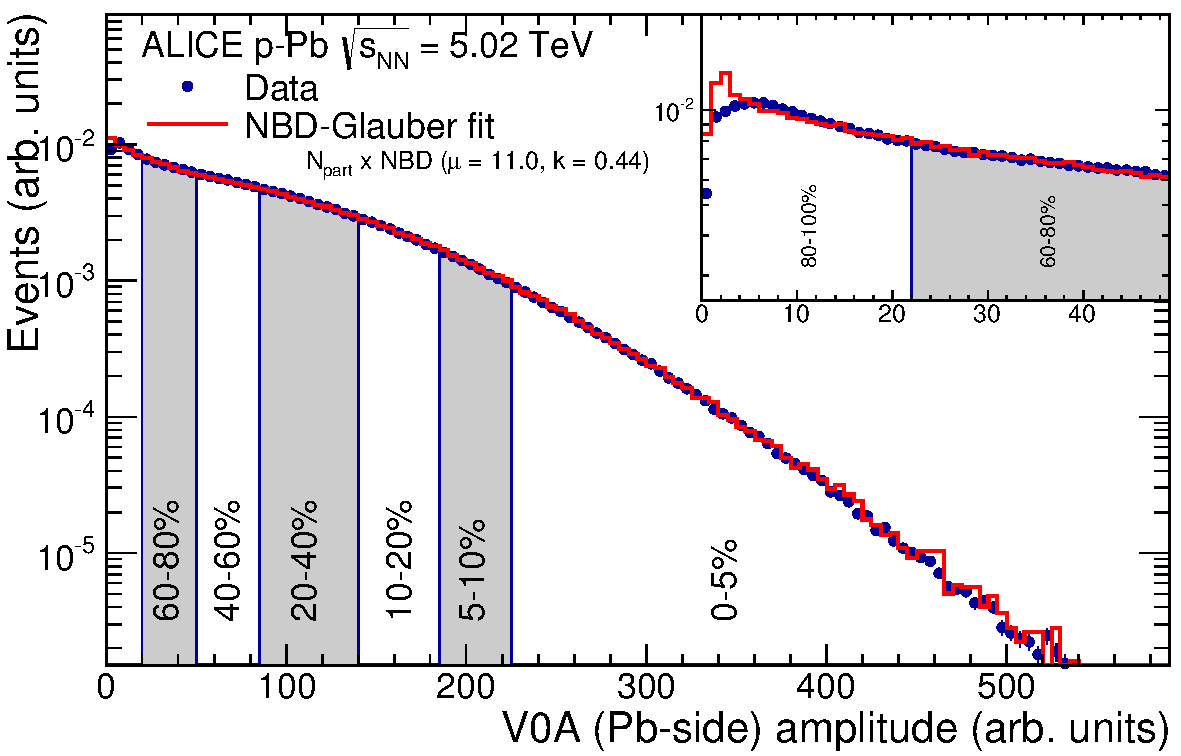
\includegraphics[width=0.50\textwidth]{pics/CentralitypPb}
                \caption{Distribution of the sum of amplitudes in the V0A hodoscopes (Pb-going), as well
as the NBD-Glauber fit (explained in the text). Centrality classes are indicated by vertical lines. The
inset shows a zoom-in on the most peripheral events.~\cite{Adam:2014qja}}
	\label{fig:pPbcentrality}
\end{figure}



\begin{figure}[b!]
\centering
            	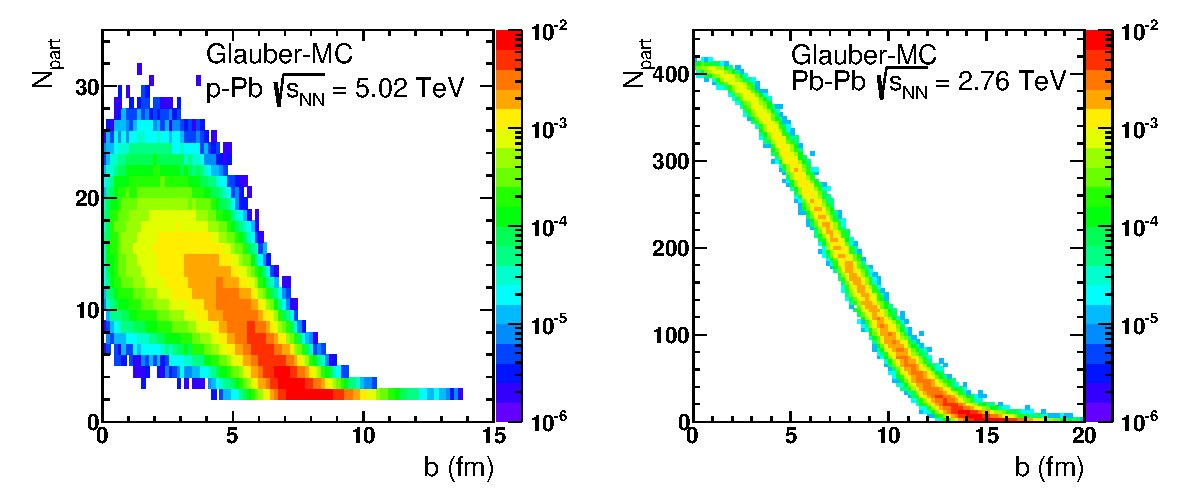
\includegraphics[width=0.9\textwidth]{pics/BNpart_Glau-10758.pdf}

            	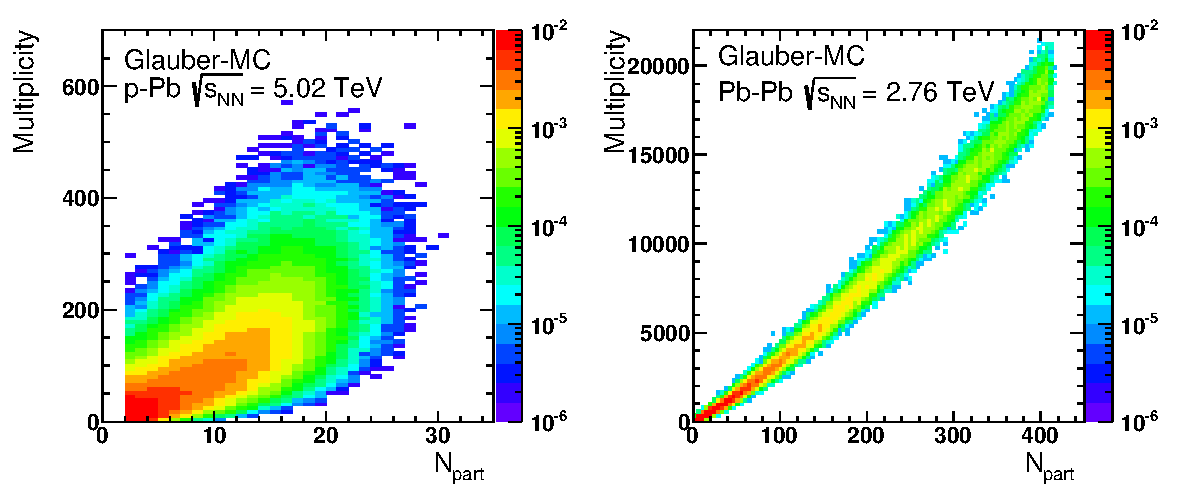
\includegraphics[width=0.9\textwidth]{pics/NpartMult_Glau-10759.pdf}
                \caption{Top: Scatter plot of number of participating nucleons versus impact parameter; Bottom: Scatter plot of multiplicity versus the number of participating nucleons from the Glauber fit for V0A. The quantities are calculated with a Glauber Monte Carlo of p-Pb (left) and Pb-Pb (right) collisions.~\cite{Adam:2014qja}}
	\label{fig:pPbMult}
\end{figure}


Additional kinematic biases exist for events containing high-$\pt{}$ particles, which arise from the fragmentation of partons produced in parton-parton scattering with large momentum transfer. Their contribution to the overall multiplicity increases with increasing parton energy and thus can introduce a trivial correlation between the centrality estimator and the presence of a high-$\pt{}$ particle in the event. For very peripheral collisions, the multiplicity range that governs the centrality for the bulk of soft collisions can represent an effective veto on hard processes. For the nuclear modification factor this would lead to $R_\mathrm{pPb} < 1$.


